\subsubsection{Dataset and event selection}
- dire run number, mc production
- dire ZNA selection
- dire numero di eventi
- in futuro: sezione V0A vs ZNA

\subsubsection{Mass plots and D-meson selection}
- dire cut optimization D0
- mostrare i mass plot

\begin{figure}[!htp]
\centering

{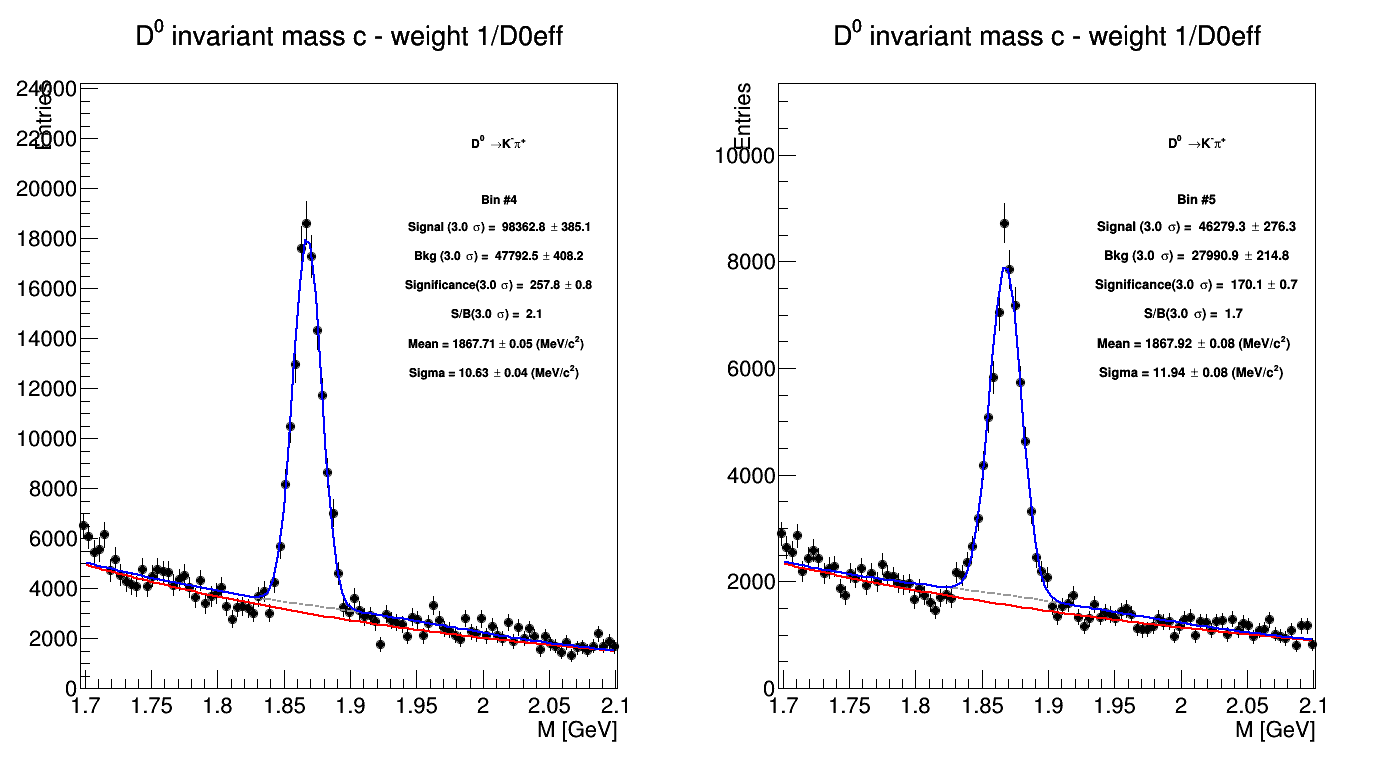
\includegraphics[width=1\linewidth, height=5.6cm]{figuresVsCent/Dzero/MassPlots/020/InvMassDistributions_Dzero_Bins4to5.png}}
{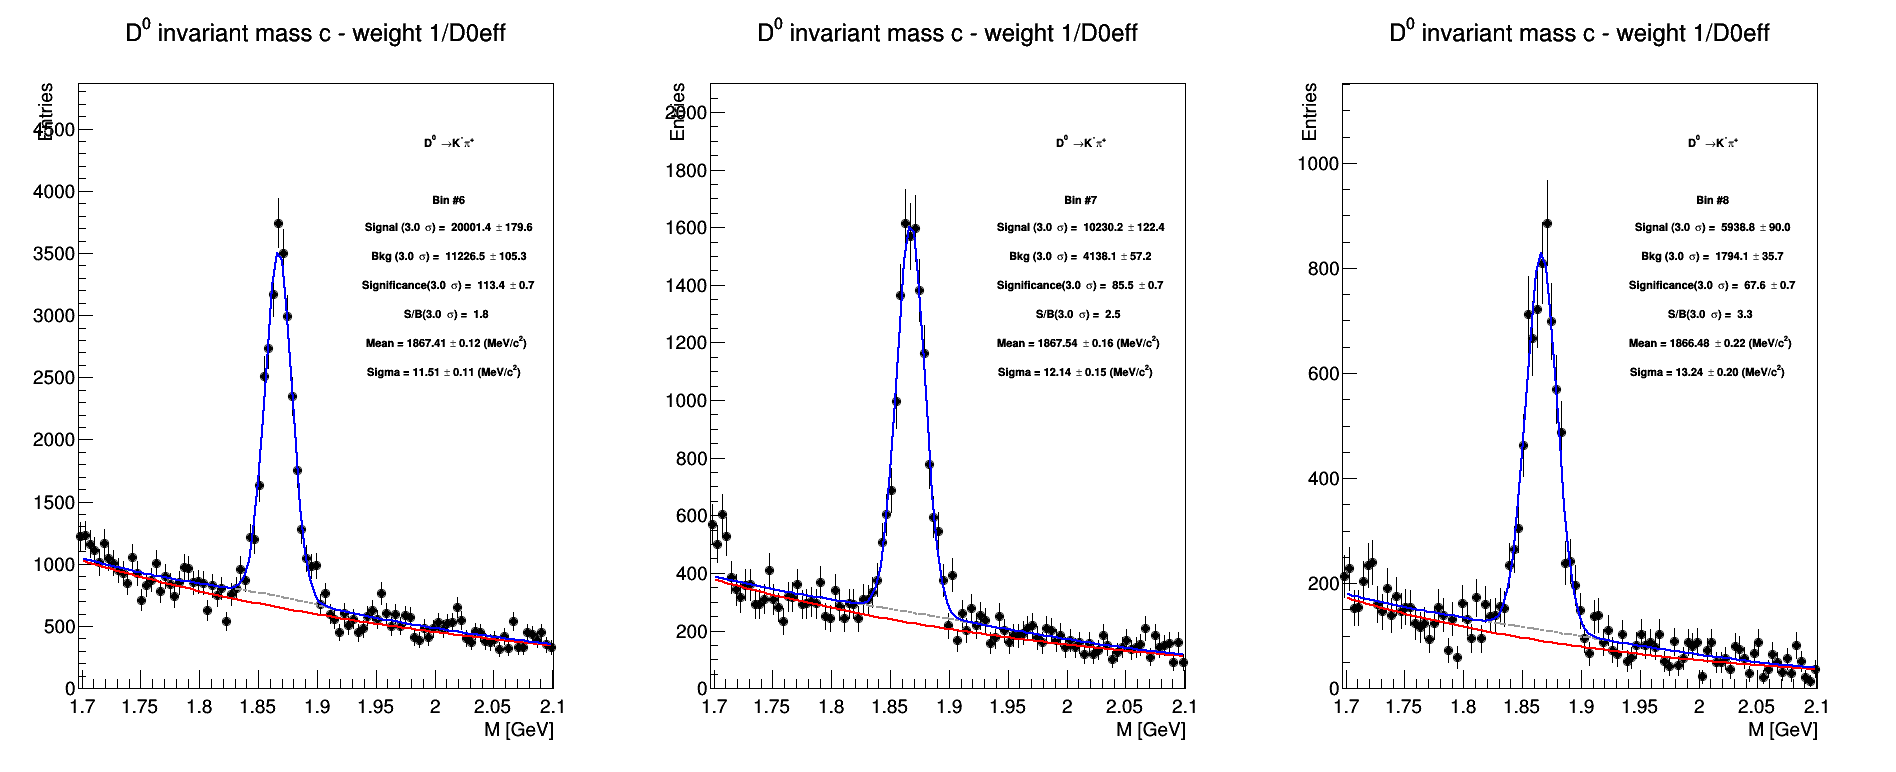
\includegraphics[width=1\linewidth, height=5.6cm]{figuresVsCent/Dzero/MassPlots/020/InvMassDistributions_Dzero_Bins6to8.png}}
{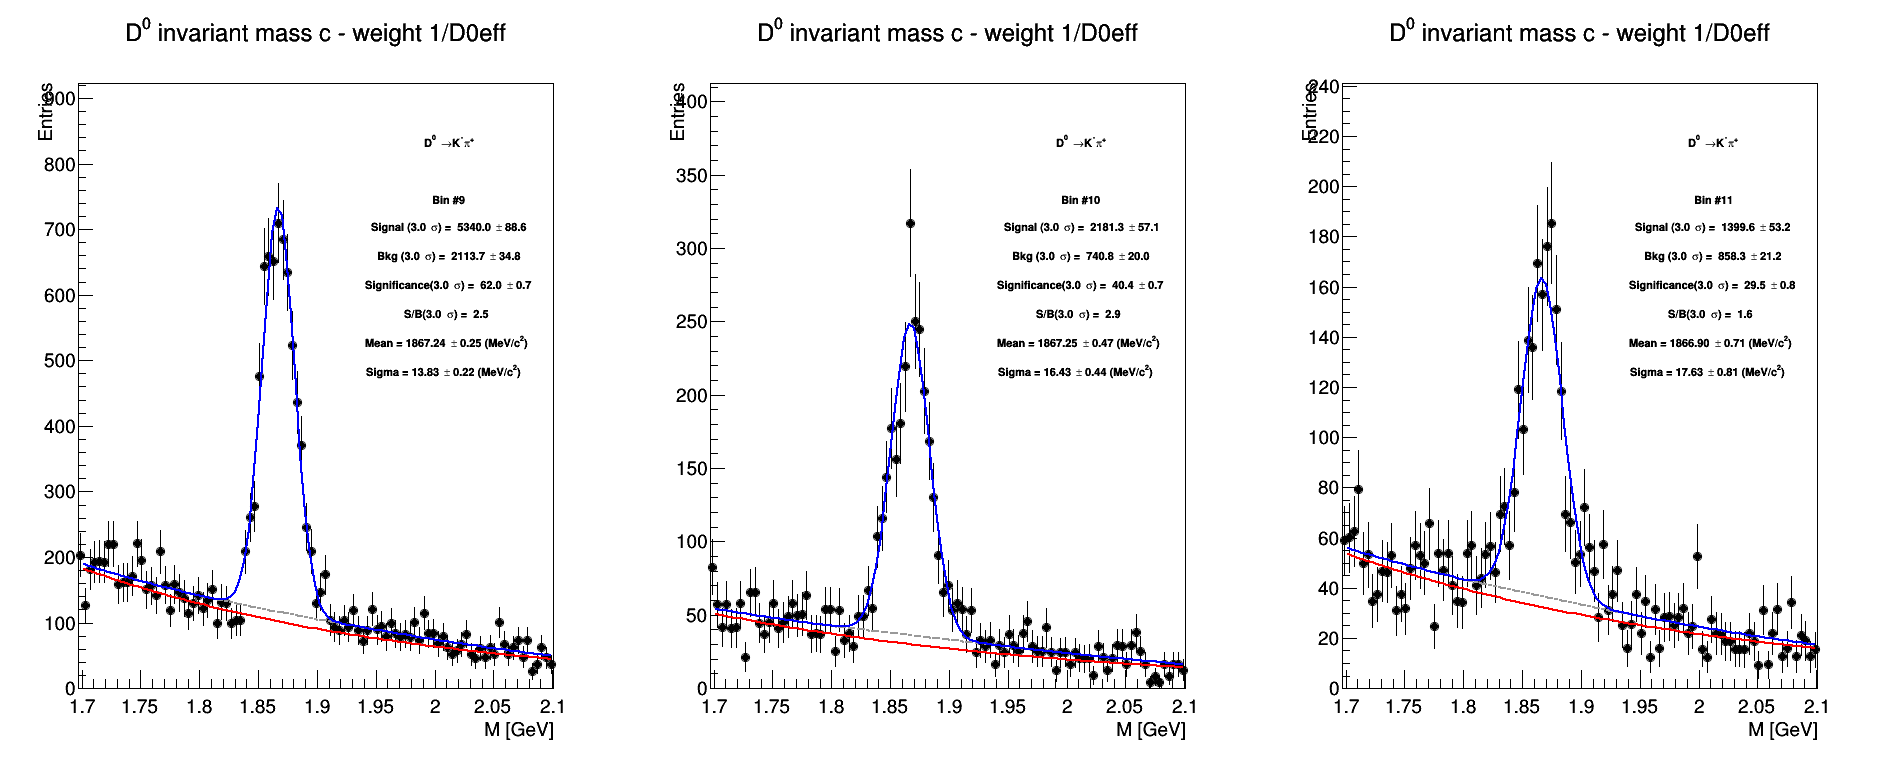
\includegraphics[width=1\linewidth, height=5.6cm]{figuresVsCent/Dzero/MassPlots/020/InvMassDistributions_Dzero_Bins9to11.png}}
{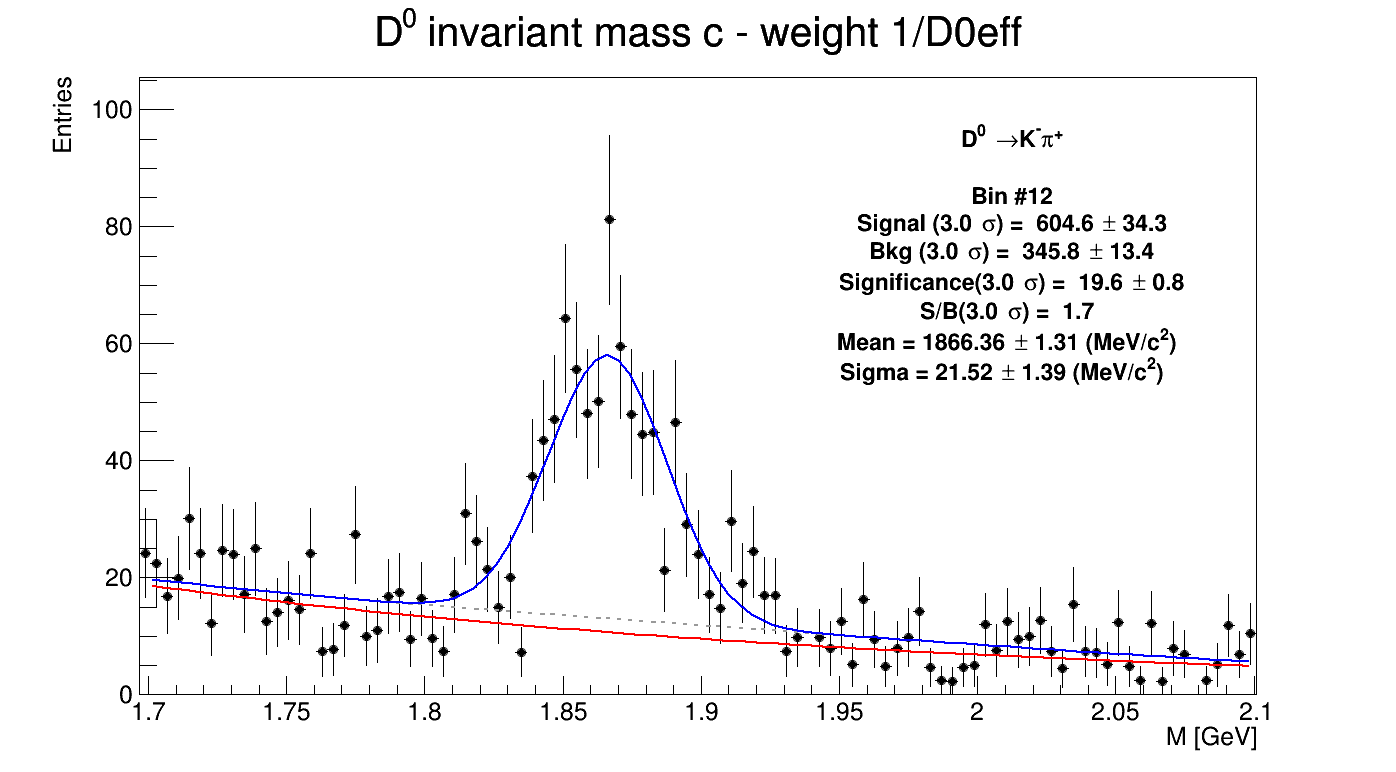
\includegraphics[width=0.6\linewidth, height=5.6cm]{figuresVsCent/Dzero/MassPlots/020/InvMassDistributions_Dzero_Bins12to12.png}}

%[width=.32\linewidth]
\caption{Invariant mass distributions of $D^0$ corrected with efficiency in different $\text{p}_T$ regions for 0-20$\%$ centrality class. Top: $3< p_{T}^{\text{D}}< 4$ $\gev/c$ (left), $4< p_{T}^{\text{D}}< 5$ $\gev/c$ right), Mid 1: $5< p_{T}^{\text{D}}< 6$ $\gev/c$ (left), $6 < p_{T}^{\text{D}} < 7$ $\gev/c$ (middle), $7< p_{T}^{\text{D}}< 8$ $\gev/c$ (right); Mid2: $8< p_{T}^{\text{D}}< 10$ $\gev/c$, $10< p_{T}^{\text{D}}< 12$ $\gev/c$  (middle), $12 < p_{T}^{\text{D}}< 16$ $\gev/c$  (right) and Bottom: $16<p_{T}^{\text{D}}< 24$ $\gev/c$.}
\label{fig:InvMassD0020}
\end{figure}


\begin{figure}[!htp]
\centering
{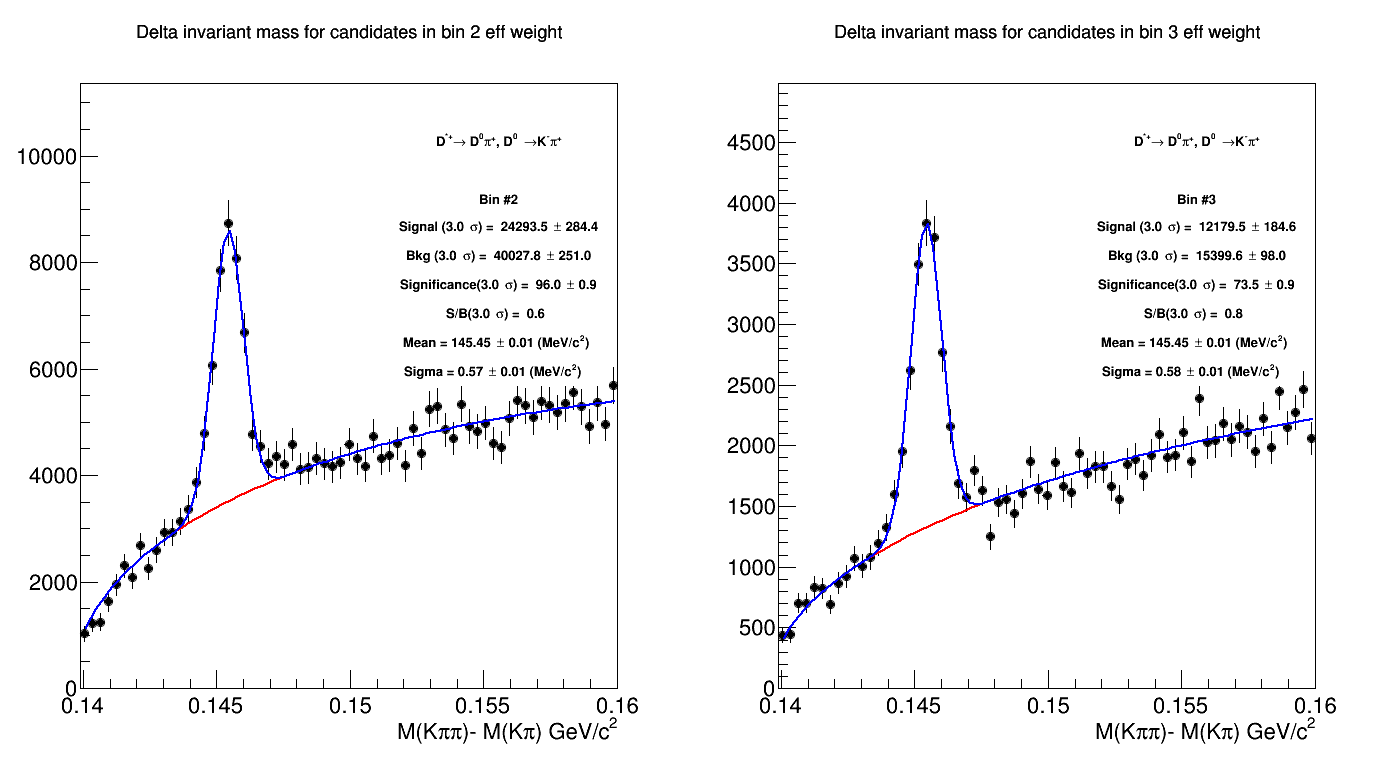
\includegraphics[width=1\linewidth, height=5.6cm]{figuresVsCent/Dstar/MassPlots/020/InvMassDistributions_Dstar_Bins2to3.png}}
{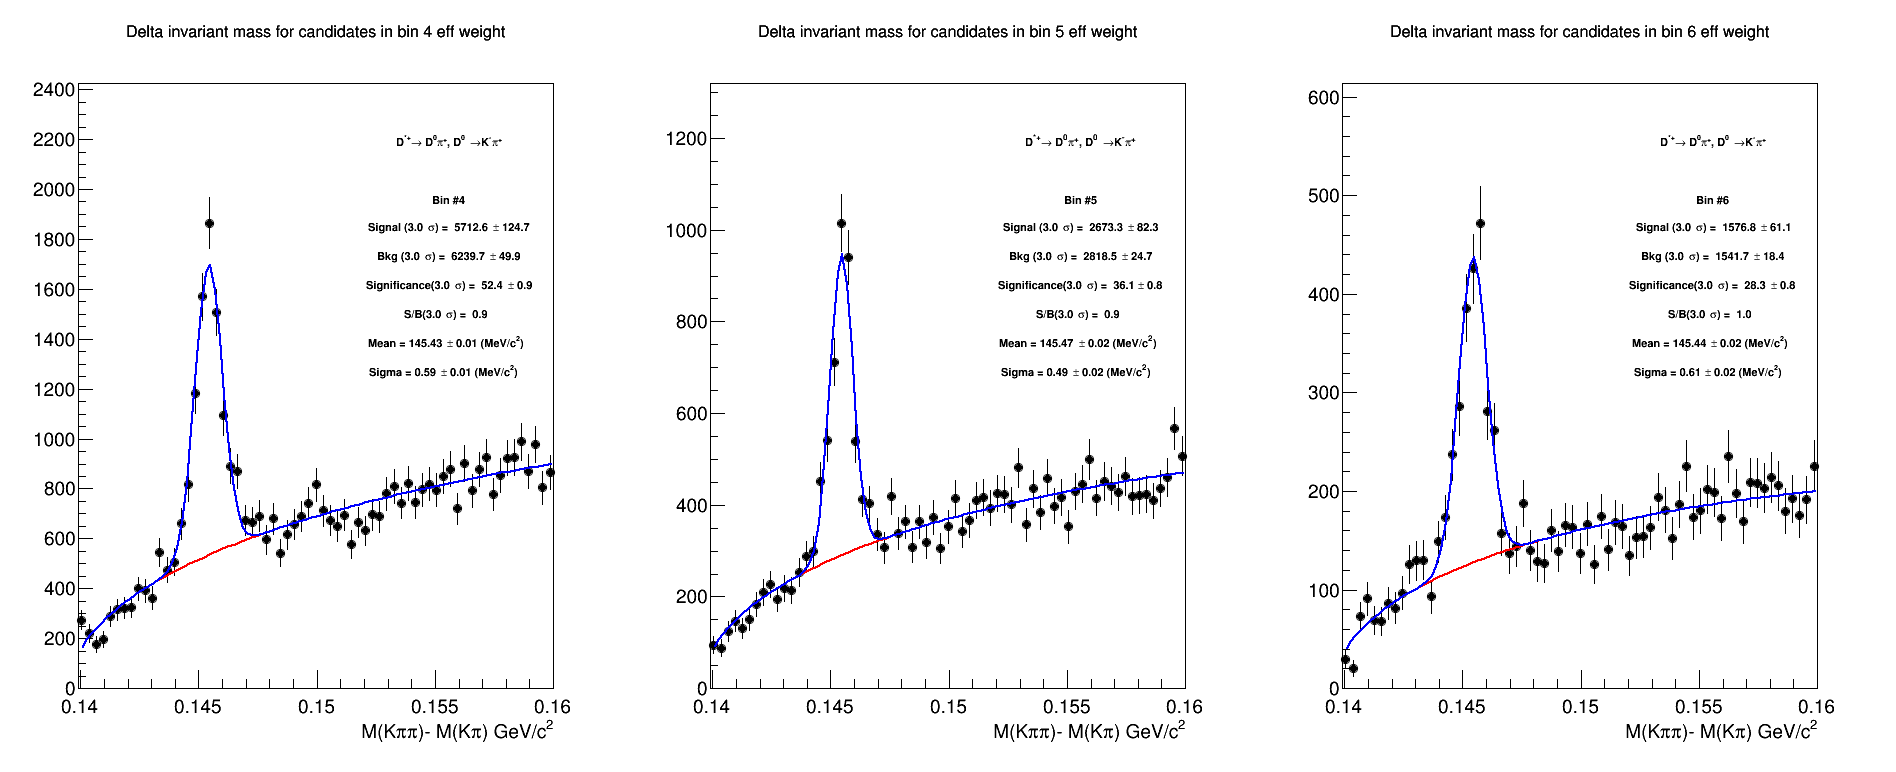
\includegraphics[width=1\linewidth, height=5.6cm]{figuresVsCent/Dstar/MassPlots/020/InvMassDistributions_Dstar_Bins4to6.png}}
{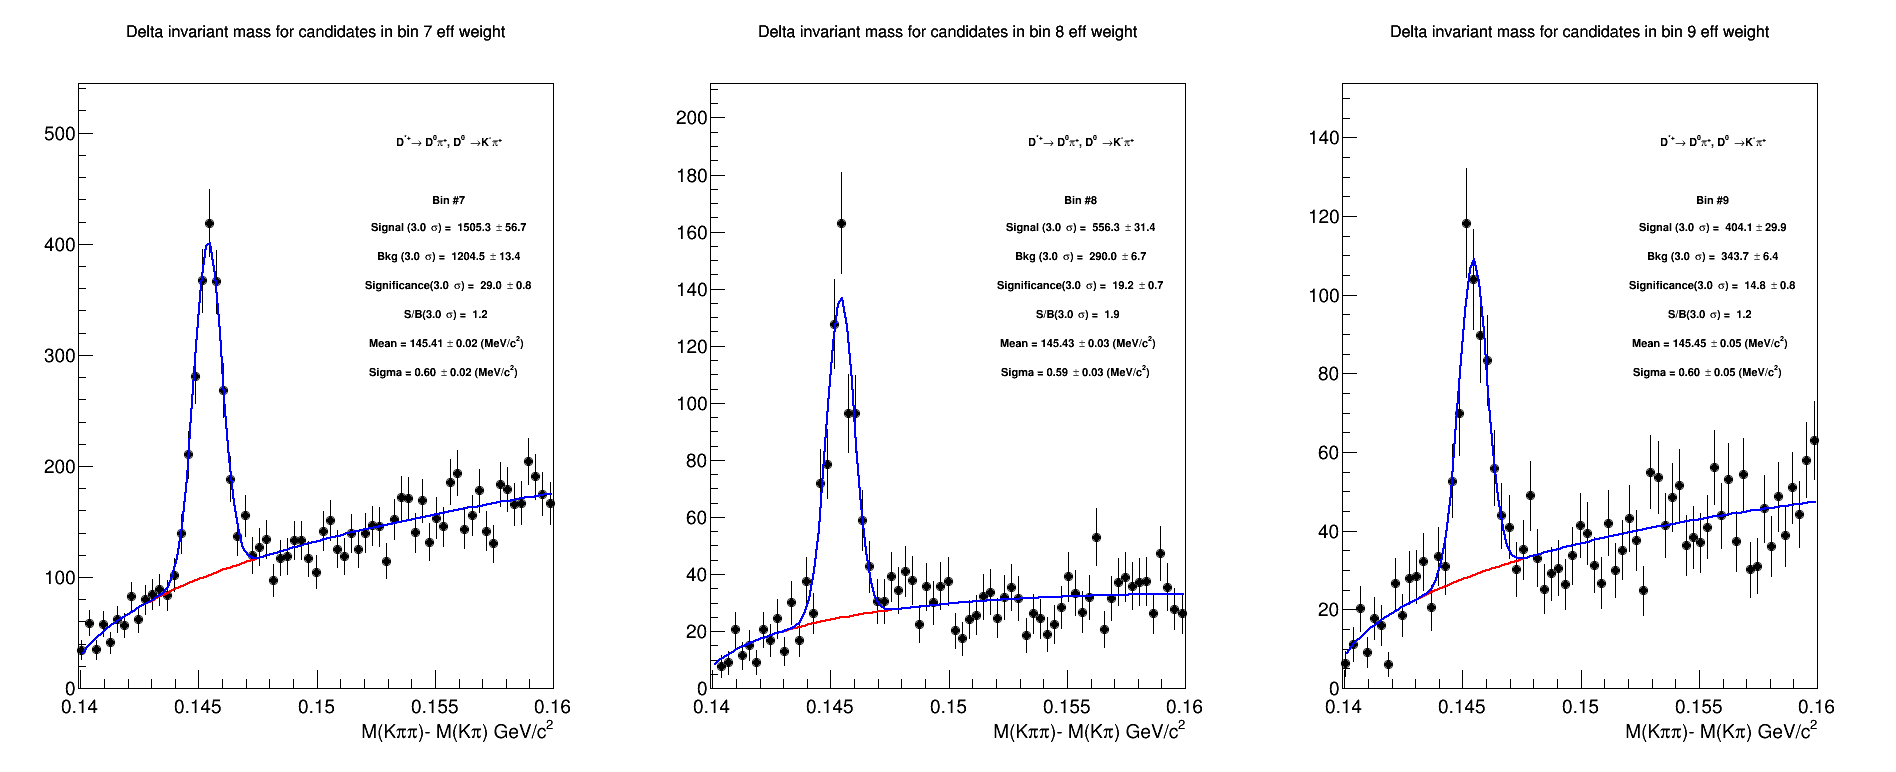
\includegraphics[width=1\linewidth, height=5.6cm]{figuresVsCent/Dstar/MassPlots/020/InvMassDistributions_Dstar_Bins7to9.png}}
{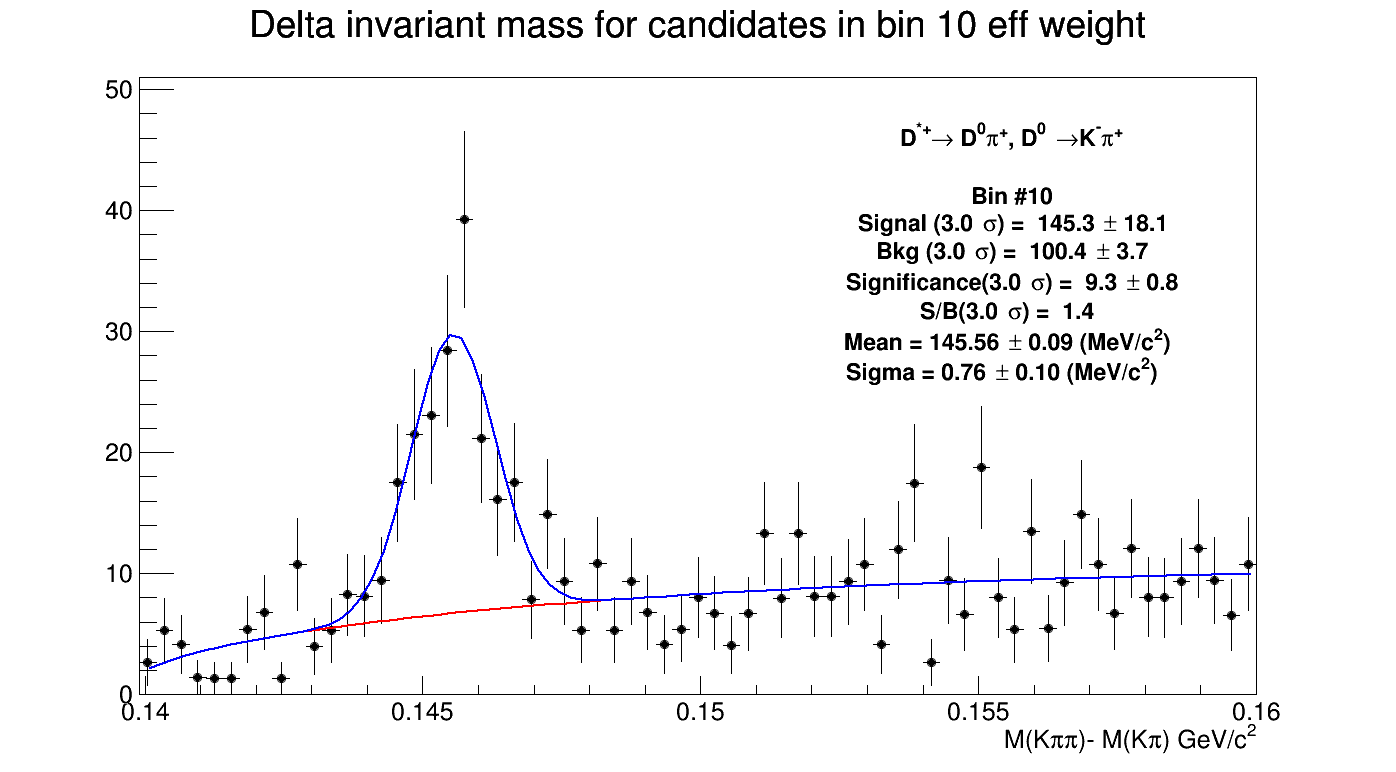
\includegraphics[width=0.6\linewidth, height=5.6cm]{figuresVsCent/Dstar/MassPlots/020/InvMassDistributions_Dstar_Bins10to10.png}}

\caption{Invariant mass distributions of $\Dstar$ corrected with efficiency in different $\text{p}_T$ regions for 0-20$\%$ centrality class. Top: $3< p_{T}^{\text{D}}< 4$ $\gev/c$ (left), $4< p_{T}^{\text{D}}< 5$ $\gev/c$ right), Mid 1: $5< p_{T}^{\text{D}}< 6$ $\gev/c$ (left), $6 < p_{T}^{\text{D}} < 7$ $\gev/c$ (middle), $7< p_{T}^{\text{D}}< 8$ $\gev/c$ (right); Mid2: $8< p_{T}^{\text{D}}< 10$ $\gev/c$, $10< p_{T}^{\text{D}}< 12$ $\gev/c$  (middle), $12 < p_{T}^{\text{D}}< 16$ $\gev/c$  (right) and Bottom: $16<p_{T}^{\text{D}}< 24$ $\gev/c$ .}
\label{fig:InvMassDs020}
\end{figure}



\begin{figure}[!htp]
\centering
{\includegraphics[width=1\linewidth, height=5.6cm]{Centrality_DPlus/Dplus/Cmp_Prompt/ZNA/0_20/DplusMassPlots/
/InvMassDistributions_Dstar_Bins3to4.png}}
{\includegraphics[width=1\linewidth, height=5.6cm]{Centrality_DPlus/Dplus/Cmp_Prompt/ZNA/0_20/DplusMassPlots/
/InvMassDistributions_Dstar_Bins5to7.png}}
{\includegraphics[width=1\linewidth, height=5.6cm]{Centrality_DPlus/Dplus/Cmp_Prompt/ZNA/0_20/DplusMassPlots/
/InvMassDistributions_Dstar_Bins8to10.png}}
{\includegraphics[width=0.6\linewidth, height=5.6cm]{Centrality_DPlus/Dplus/Cmp_Prompt/ZNA/0_20/DplusMassPlots/
/InvMassDistributions_Dstar_Bins11to11.png}}

\caption{Invariant mass distributions of $\Dplus$ corrected with efficiency in different $\text{p}_T$ regions for 0-20$\%$ centrality class. Top: $3< p_{T}^{\text{D}}< 4$ $\gev/c$ (left), $4< p_{T}^{\text{D}}< 5$ $\gev/c$ right), Mid 1: $5< p_{T}^{\text{D}}< 6$ $\gev/c$ (left), $6 < p_{T}^{\text{D}} < 7$ $\gev/c$ (middle), $7< p_{T}^{\text{D}}< 8$ $\gev/c$ (right); Mid2: $8< p_{T}^{\text{D}}< 10$ $\gev/c$, $10< p_{T}^{\text{D}}< 12$ $\gev/c$  (middle), $12 < p_{T}^{\text{D}}< 16$ $\gev/c$  (right) and Bottom: $16<p_{T}^{\text{D}}< 24$ $\gev/c$ .}
\label{fig:InvMassDplus020}
\end{figure}

\begin{figure}[!htp]
\centering

{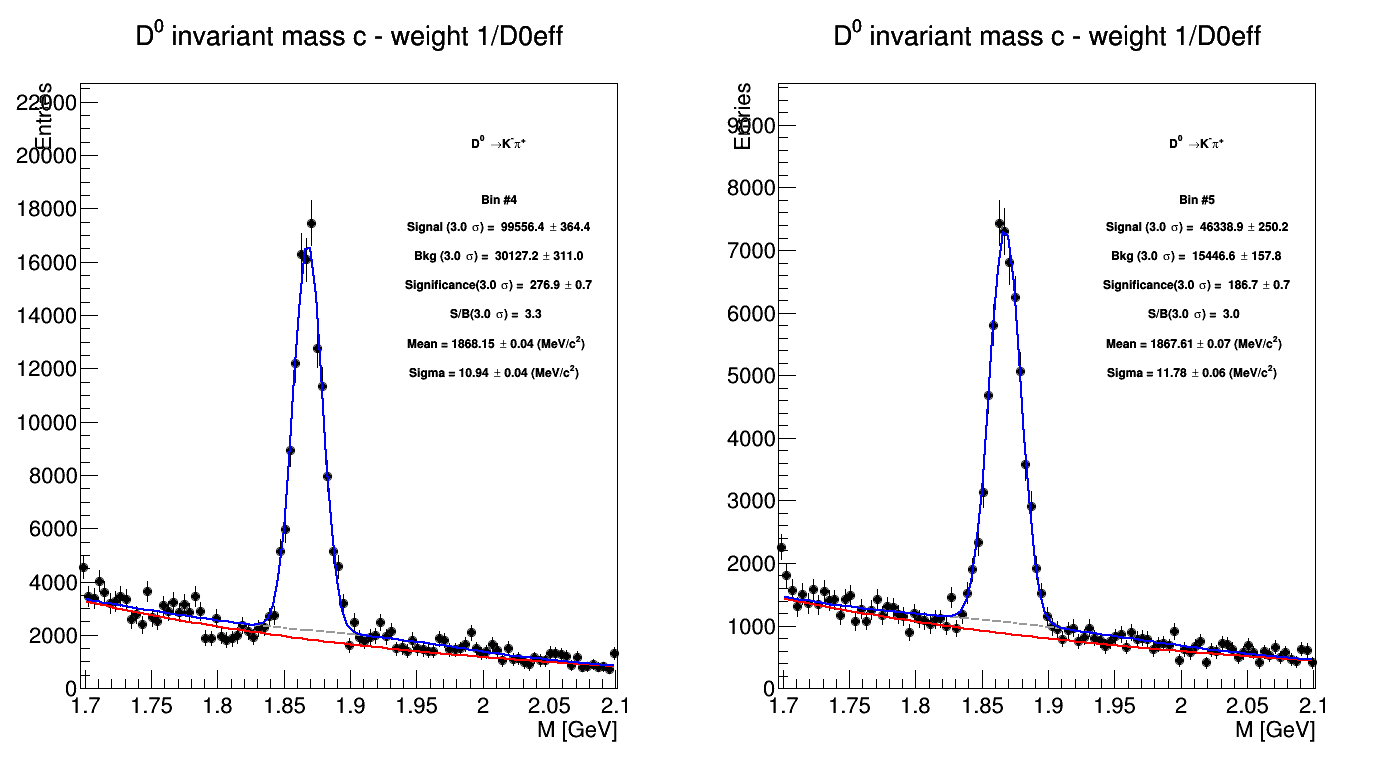
\includegraphics[width=1\linewidth, height=5.6cm]{figuresVsCent/Dzero/MassPlots/2060/InvMassDistributions_Dzero_Bins4to5.png}}
{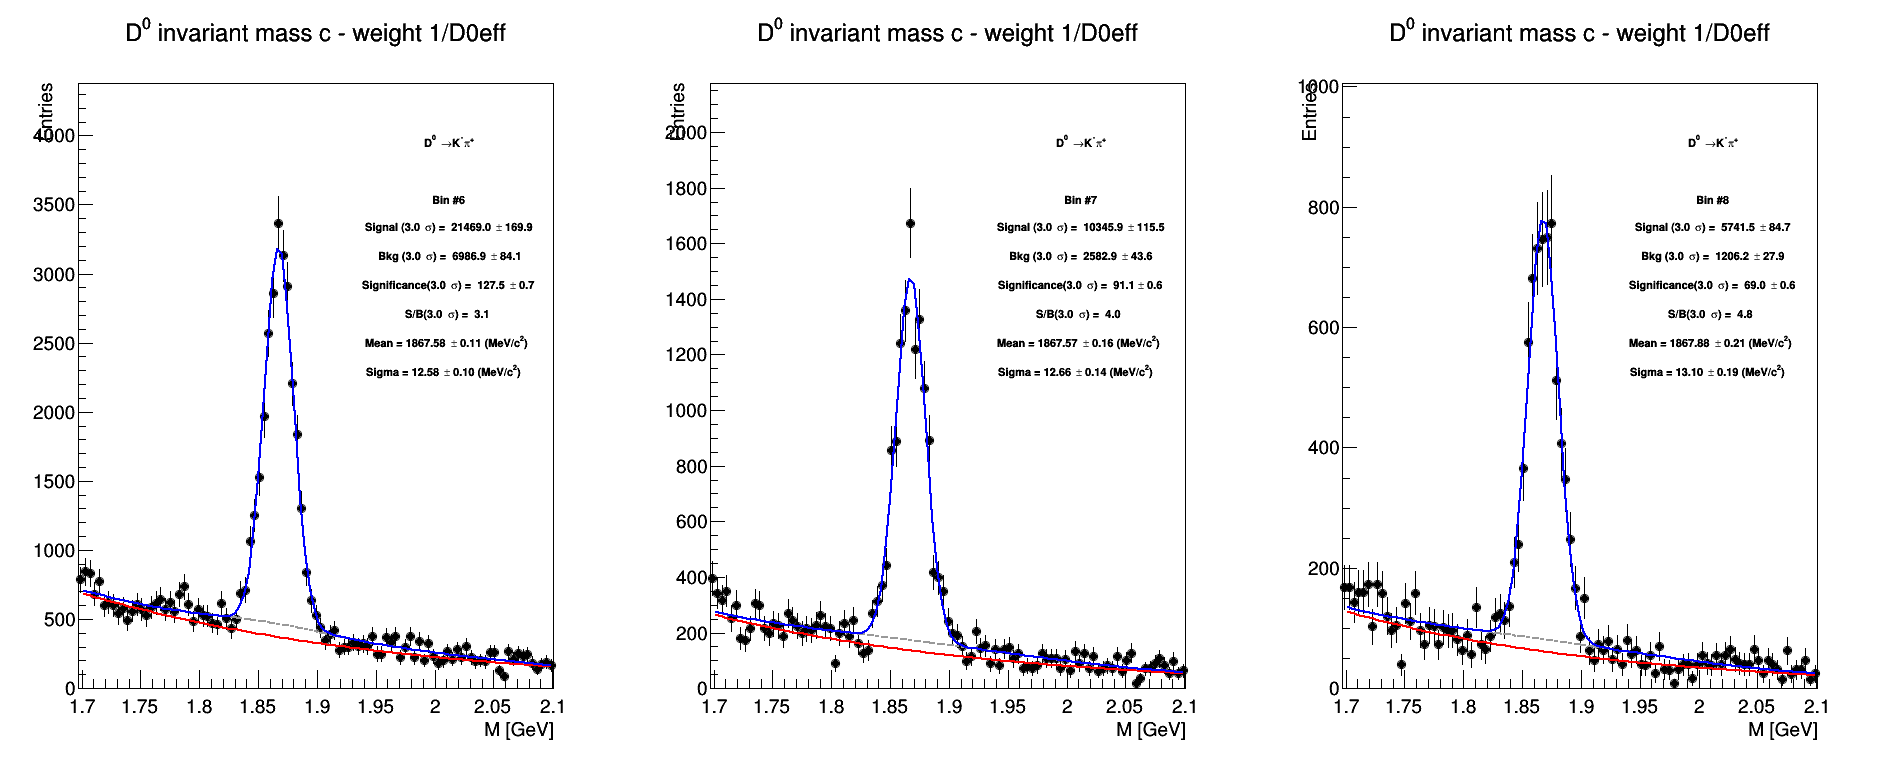
\includegraphics[width=1\linewidth, height=5.6cm]{figuresVsCent/Dzero/MassPlots/2060/InvMassDistributions_Dzero_Bins6to8.png}}
{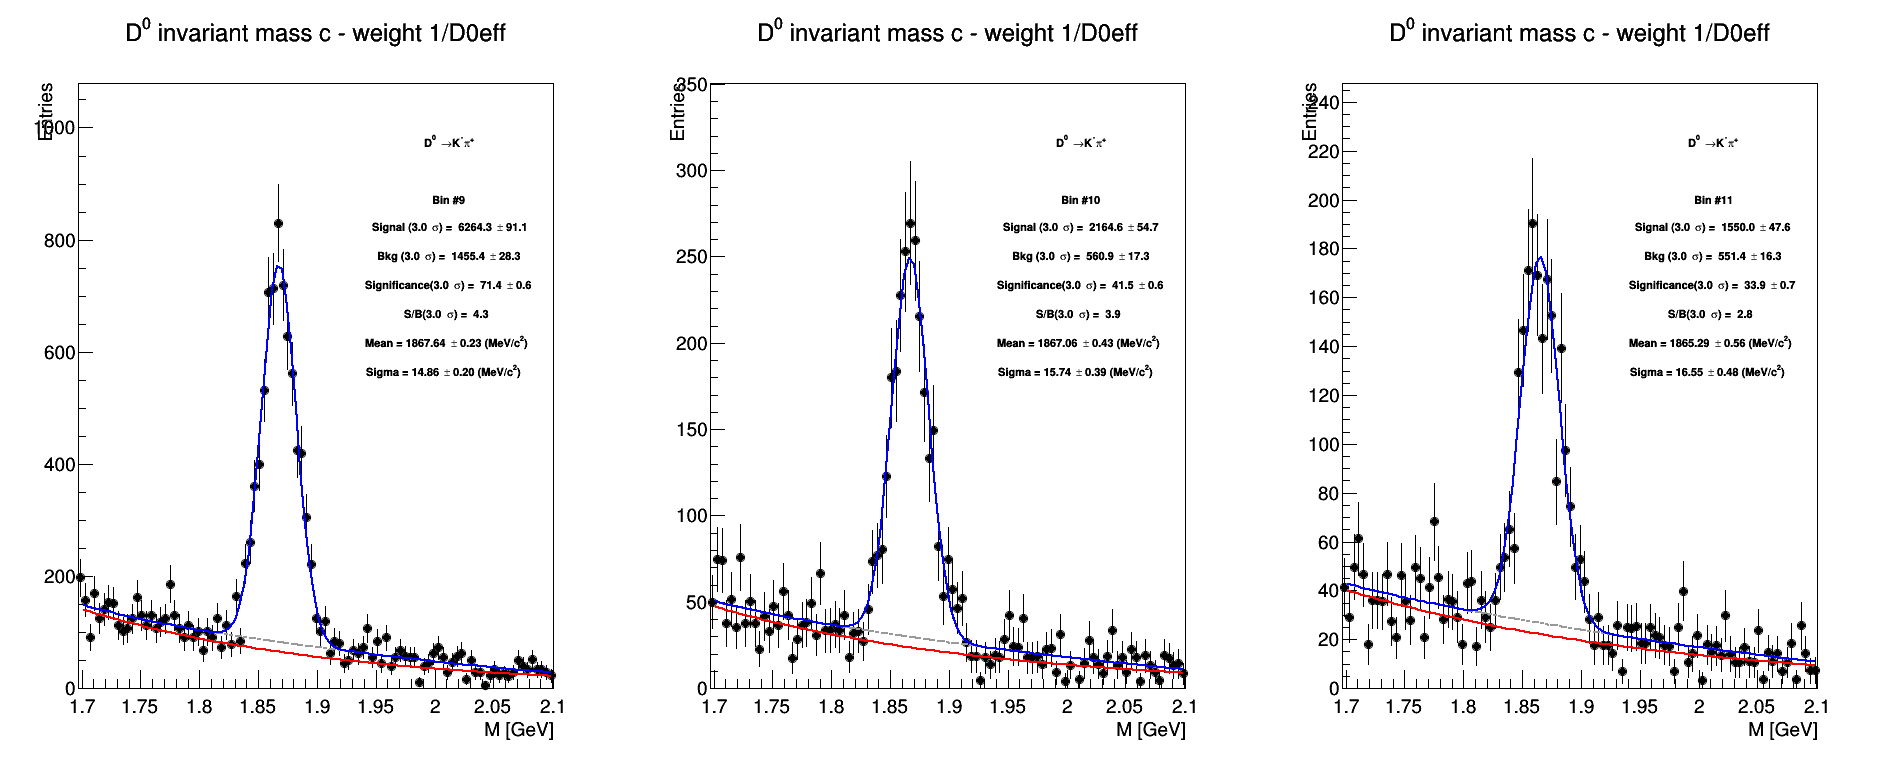
\includegraphics[width=1\linewidth, height=5.6cm]{figuresVsCent/Dzero/MassPlots/2060/InvMassDistributions_Dzero_Bins9to11.png}}
{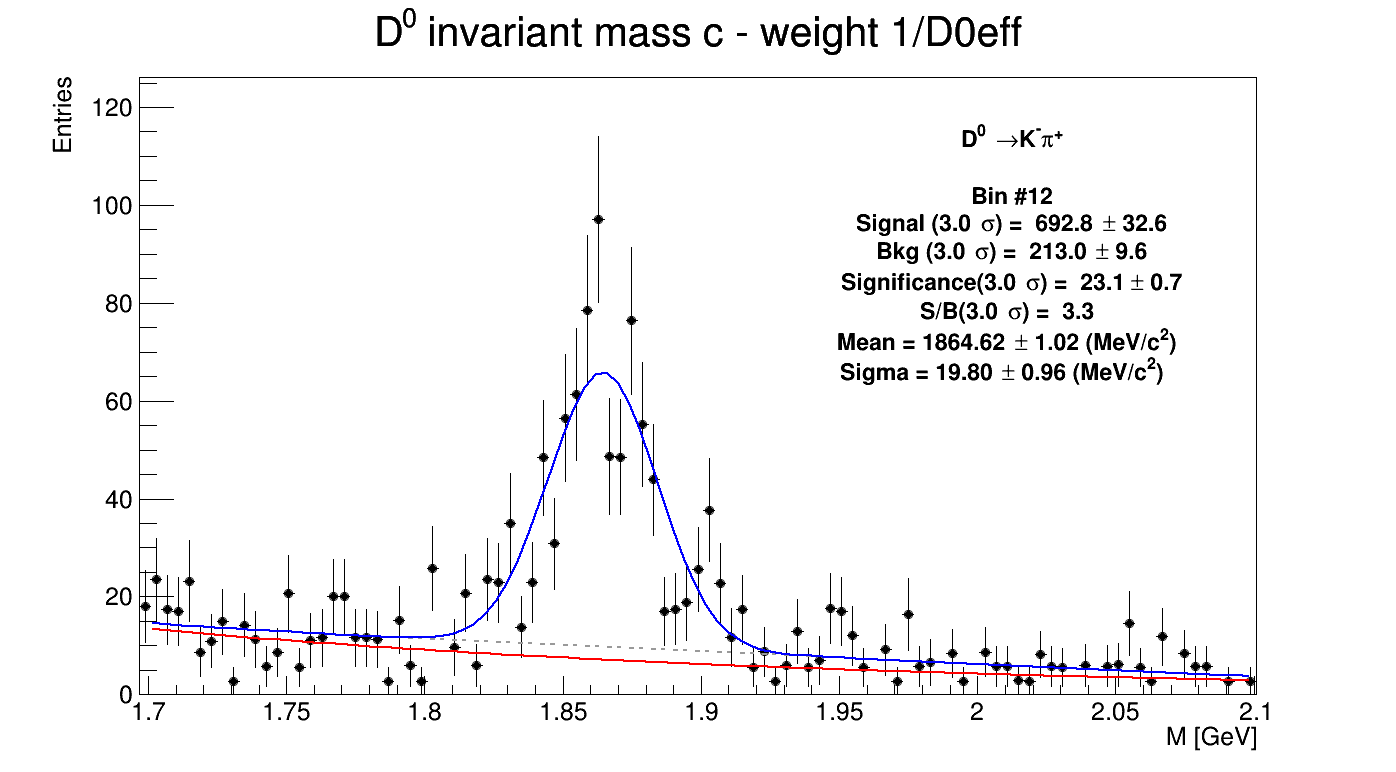
\includegraphics[width=0.6\linewidth, height=5.6cm]{figuresVsCent/Dzero/MassPlots/2060/InvMassDistributions_Dzero_Bins12to12.png}}

%[width=.32\linewidth]
\caption{Invariant mass distributions of $D^0$ corrected with efficiency in different $\text{p}_T$ regions for 20-60$\%$ centrality class. Top: $3< p_{T}^{\text{D}}< 4$ $\gev/c$ (left), $4< p_{T}^{\text{D}}< 5$ $\gev/c$ right), Mid 1: $5< p_{T}^{\text{D}}< 6$ $\gev/c$ (left), $6 < p_{T}^{\text{D}} < 7$ $\gev/c$ (middle), $7< p_{T}^{\text{D}}< 8$ $\gev/c$ (right); Mid2: $8< p_{T}^{\text{D}}< 10$ $\gev/c$, $10< p_{T}^{\text{D}}< 12$ $\gev/c$  (middle), $12 < p_{T}^{\text{D}}< 16$ $\gev/c$  (right) and Bottom: $16<p_{T}^{\text{D}}< 24$ $\gev/c$.}
\label{fig:InvMassD02060}
\end{figure}


\begin{figure}[!htp]
\centering
{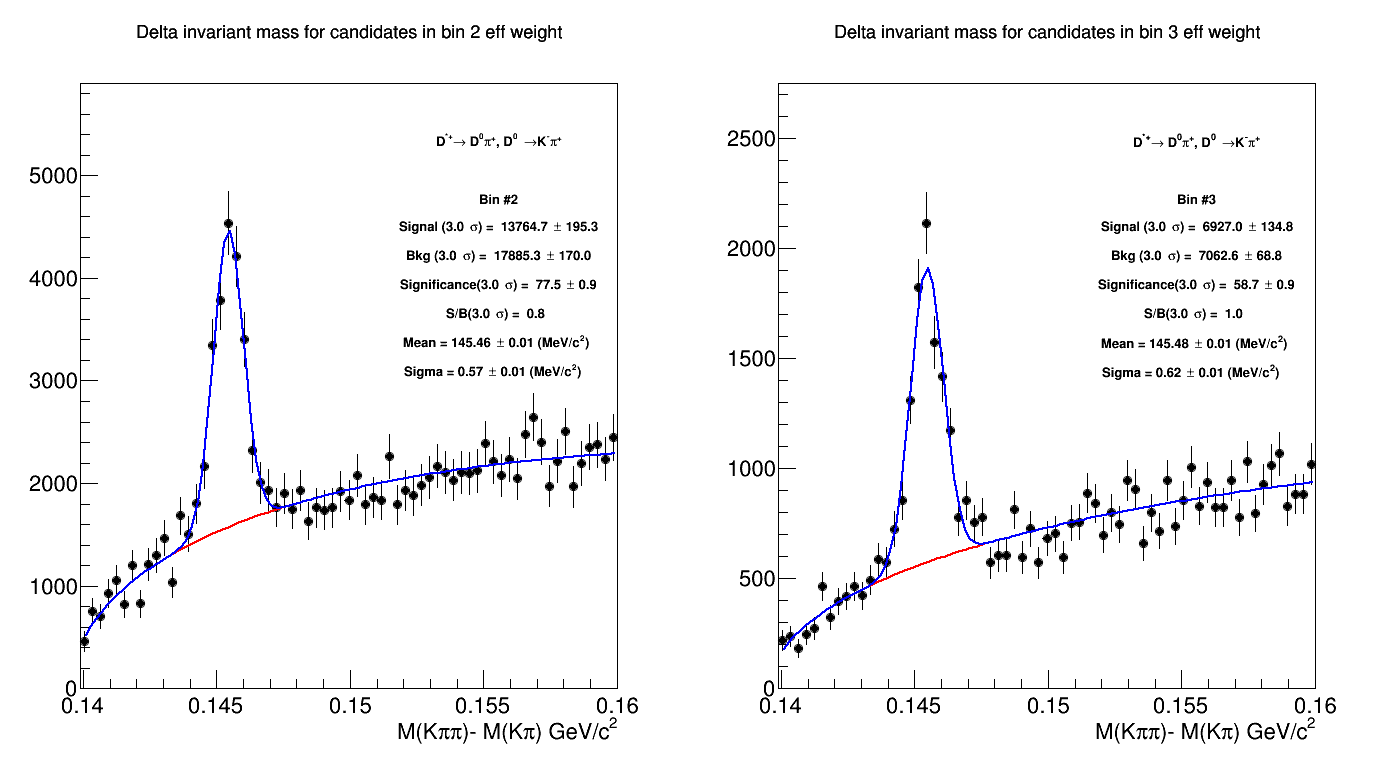
\includegraphics[width=1\linewidth, height=5.6cm]{figuresVsCent/Dstar/MassPlots/2060/InvMassDistributions_Dstar_Bins2to3.png}}
{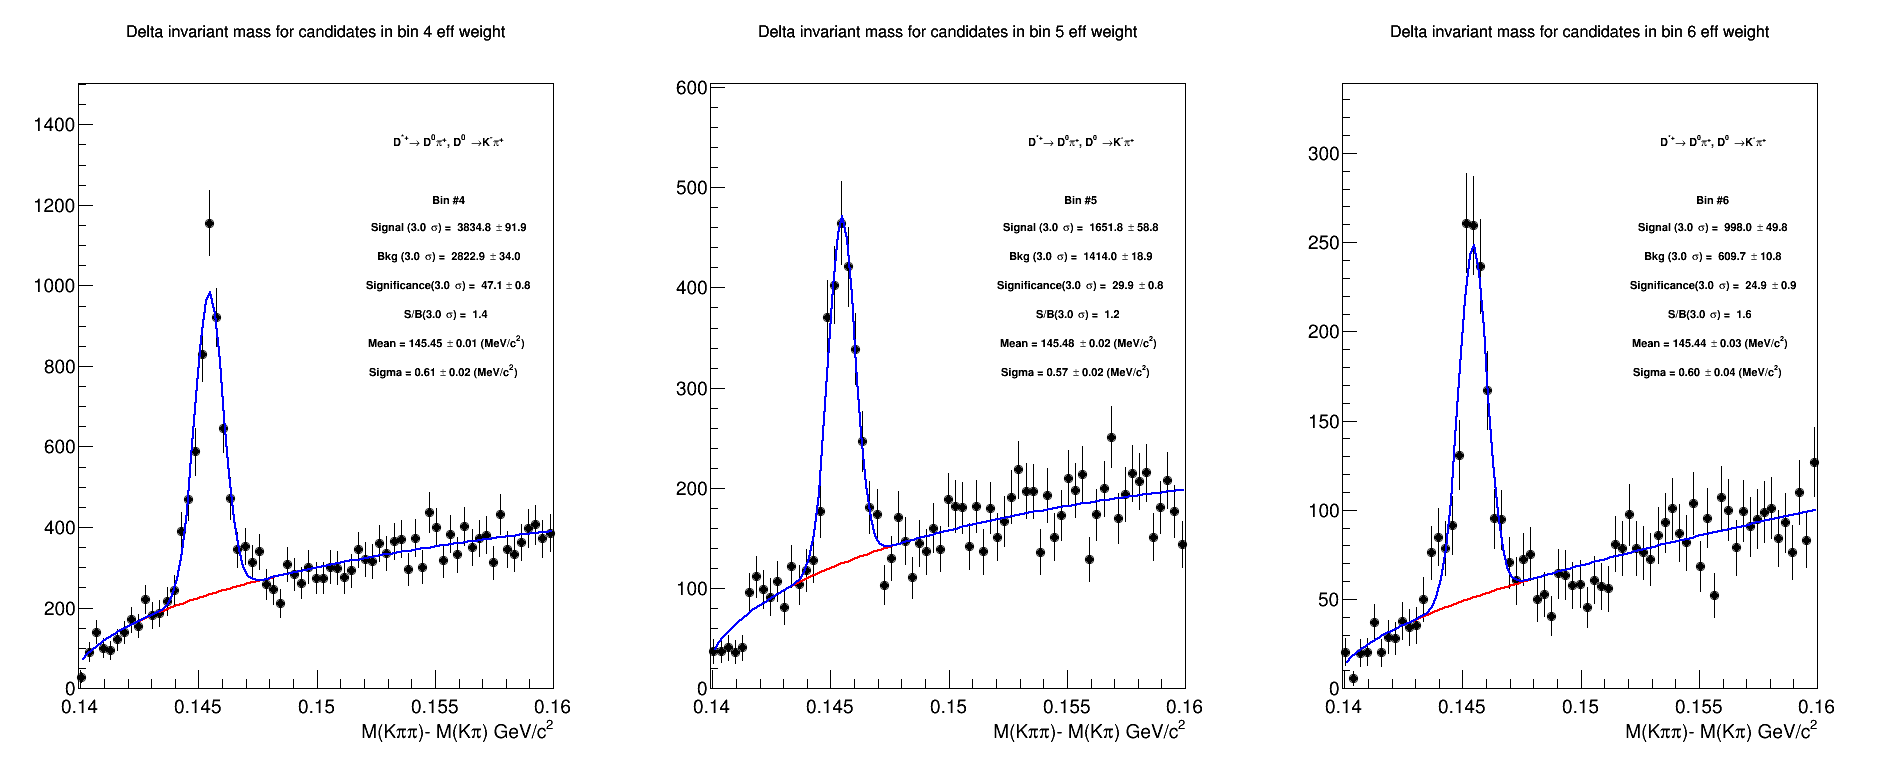
\includegraphics[width=1\linewidth, height=5.6cm]{figuresVsCent/Dstar/MassPlots/2060/InvMassDistributions_Dstar_Bins4to6.png}}
{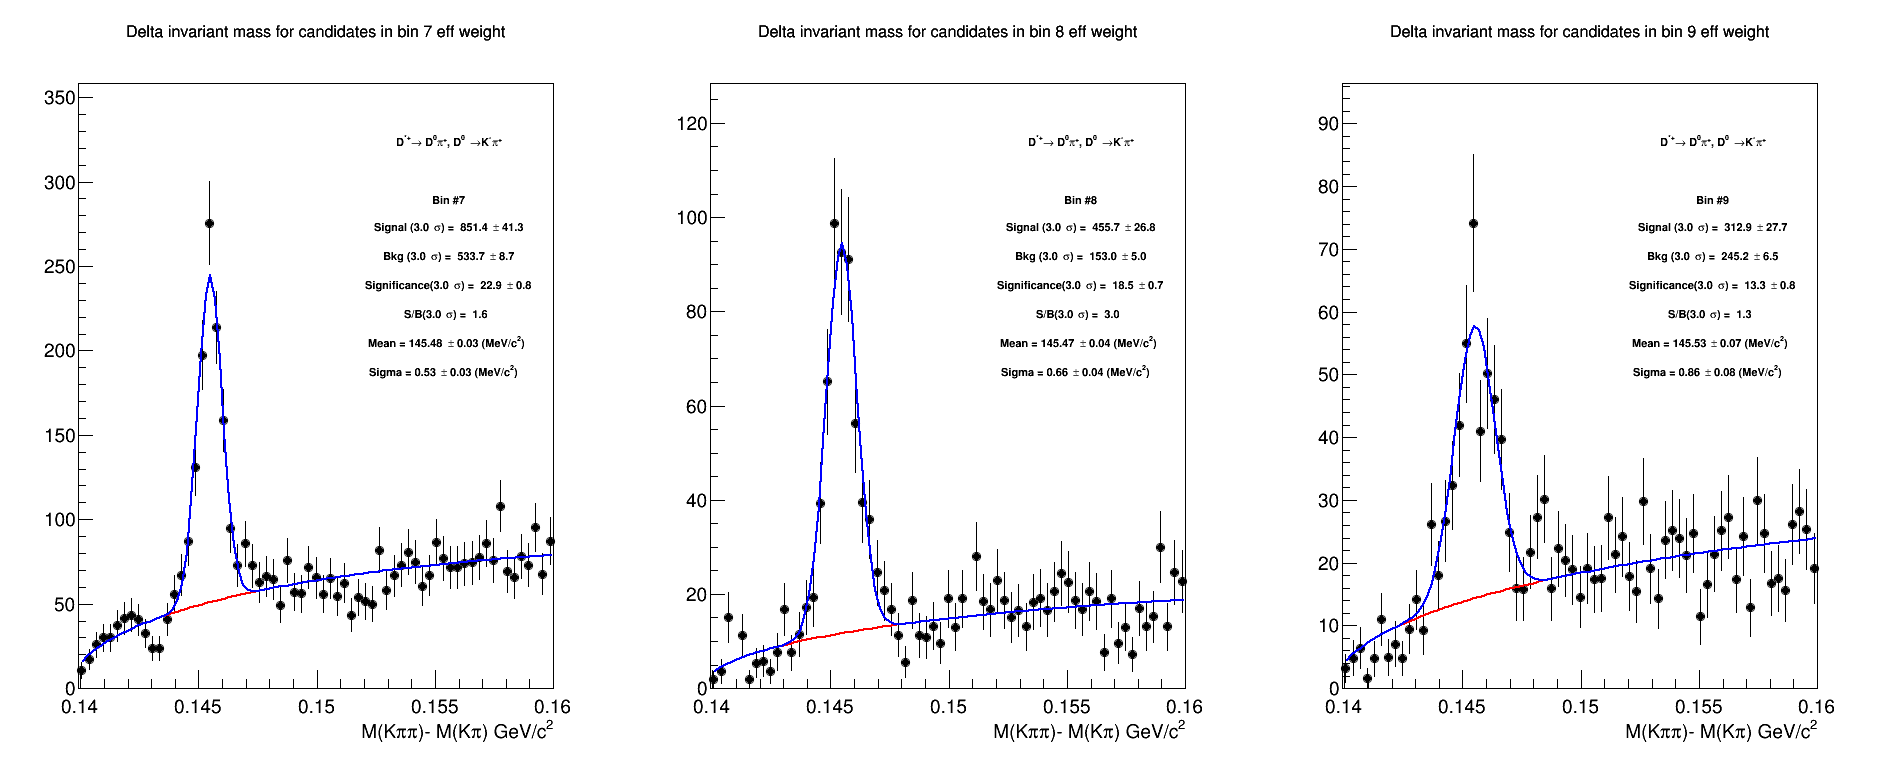
\includegraphics[width=1\linewidth, height=5.6cm]{figuresVsCent/Dstar/MassPlots/2060/InvMassDistributions_Dstar_Bins7to9.png}}
{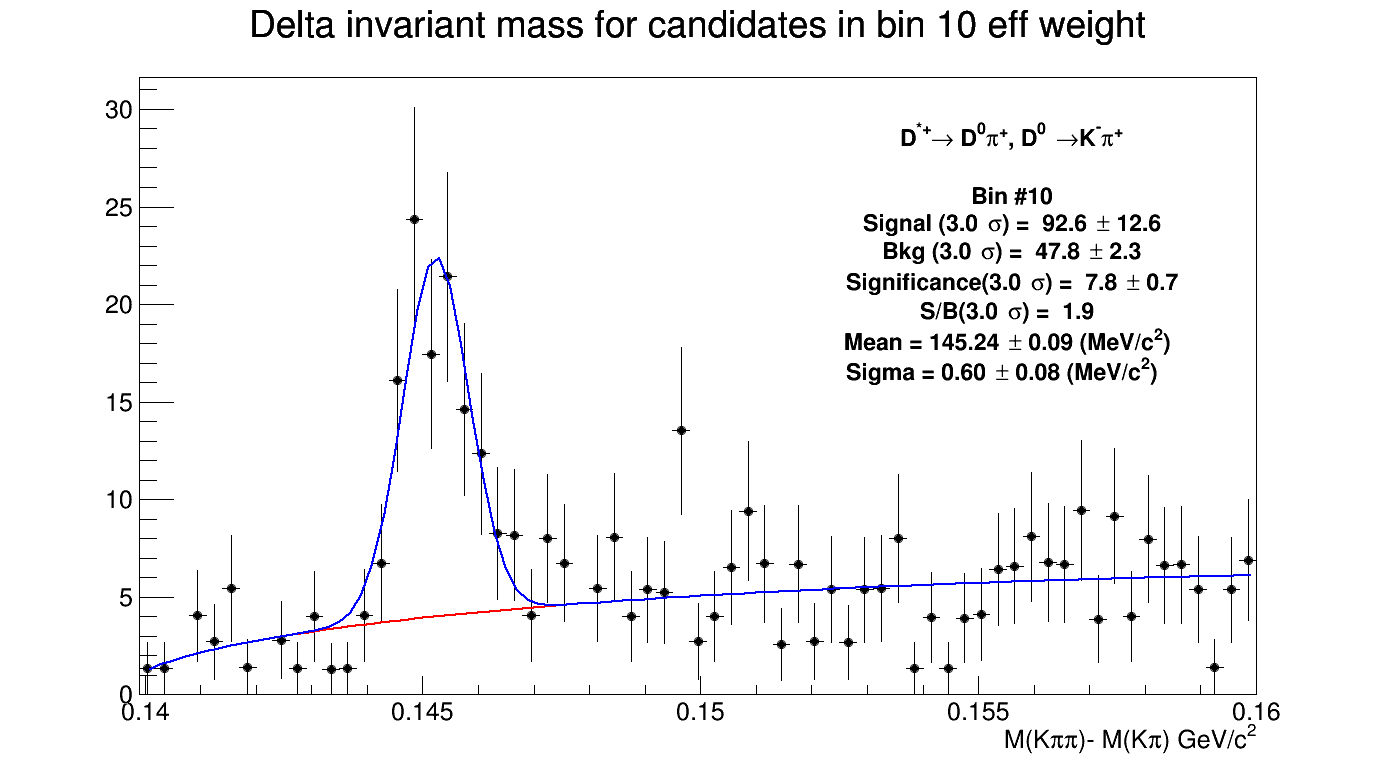
\includegraphics[width=0.6\linewidth, height=5.6cm]{figuresVsCent/Dstar/MassPlots/2060/InvMassDistributions_Dstar_Bins10to10.png}}

\caption{Invariant mass distributions of $\Dstar$ corrected with efficiency in different $\text{p}_T$ regions for 20-60$\%$ centrality class. Top: $3< p_{T}^{\text{D}}< 4$ $\gev/c$ (left), $4< p_{T}^{\text{D}}< 5$ $\gev/c$ right), Mid 1: $5< p_{T}^{\text{D}}< 6$ $\gev/c$ (left), $6 < p_{T}^{\text{D}} < 7$ $\gev/c$ (middle), $7< p_{T}^{\text{D}}< 8$ $\gev/c$ (right); Mid2: $8< p_{T}^{\text{D}}< 10$ $\gev/c$, $10< p_{T}^{\text{D}}< 12$ $\gev/c$  (middle), $12 < p_{T}^{\text{D}}< 16$ $\gev/c$  (right) and Bottom: $16<p_{T}^{\text{D}}< 24$ $\gev/c$ .}
\label{fig:InvMassDs2060}
\end{figure}



\begin{figure}[!htp]
\centering
{\includegraphics[width=1\linewidth, height=5.6cm]{Centrality_DPlus/Dplus/Cmp_Prompt/ZNA/20_60/DplusMassPlots/
/InvMassDistributions_Dstar_Bins3to4.png}}
{\includegraphics[width=1\linewidth, height=5.6cm]{Centrality_DPlus/Dplus/Cmp_Prompt/ZNA/20_60/DplusMassPlots/
/InvMassDistributions_Dstar_Bins5to7.png}}
{\includegraphics[width=1\linewidth, height=5.6cm]{Centrality_DPlus/Dplus/Cmp_Prompt/ZNA/20_60/DplusMassPlots/
/InvMassDistributions_Dstar_Bins8to10.png}}
{\includegraphics[width=0.6\linewidth, height=5.6cm]{Centrality_DPlus/Dplus/Cmp_Prompt/ZNA/20_60/DplusMassPlots/
/InvMassDistributions_Dstar_Bins11to11.png}}

\caption{Invariant mass distributions of $\Dplus$ corrected with efficiency in different $\text{p}_T$ regions for 20-60$\%$ centrality class. Top: $3< p_{T}^{\text{D}}< 4$ $\gev/c$ (left), $4< p_{T}^{\text{D}}< 5$ $\gev/c$ right), Mid 1: $5< p_{T}^{\text{D}}< 6$ $\gev/c$ (left), $6 < p_{T}^{\text{D}} < 7$ $\gev/c$ (middle), $7< p_{T}^{\text{D}}< 8$ $\gev/c$ (right); Mid2: $8< p_{T}^{\text{D}}< 10$ $\gev/c$, $10< p_{T}^{\text{D}}< 12$ $\gev/c$  (middle), $12 < p_{T}^{\text{D}}< 16$ $\gev/c$  (right) and Bottom: $16<p_{T}^{\text{D}}< 24$ $\gev/c$ .}
\label{fig:InvMassDplus2060}
\end{figure}

\begin{figure}[!htp]
\centering

{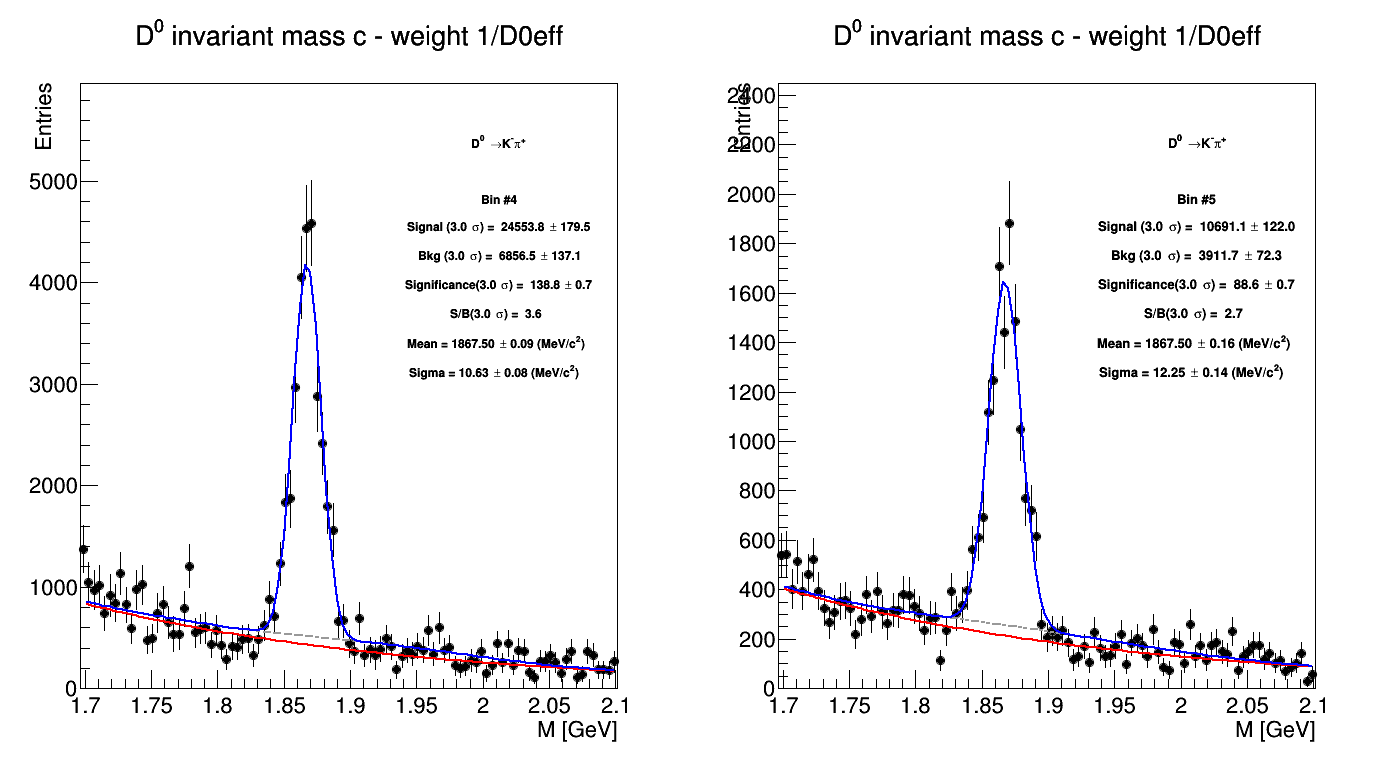
\includegraphics[width=1\linewidth, height=5.6cm]{figuresVsCent/Dzero/MassPlots/60100/InvMassDistributions_Dzero_Bins4to5.png}}
{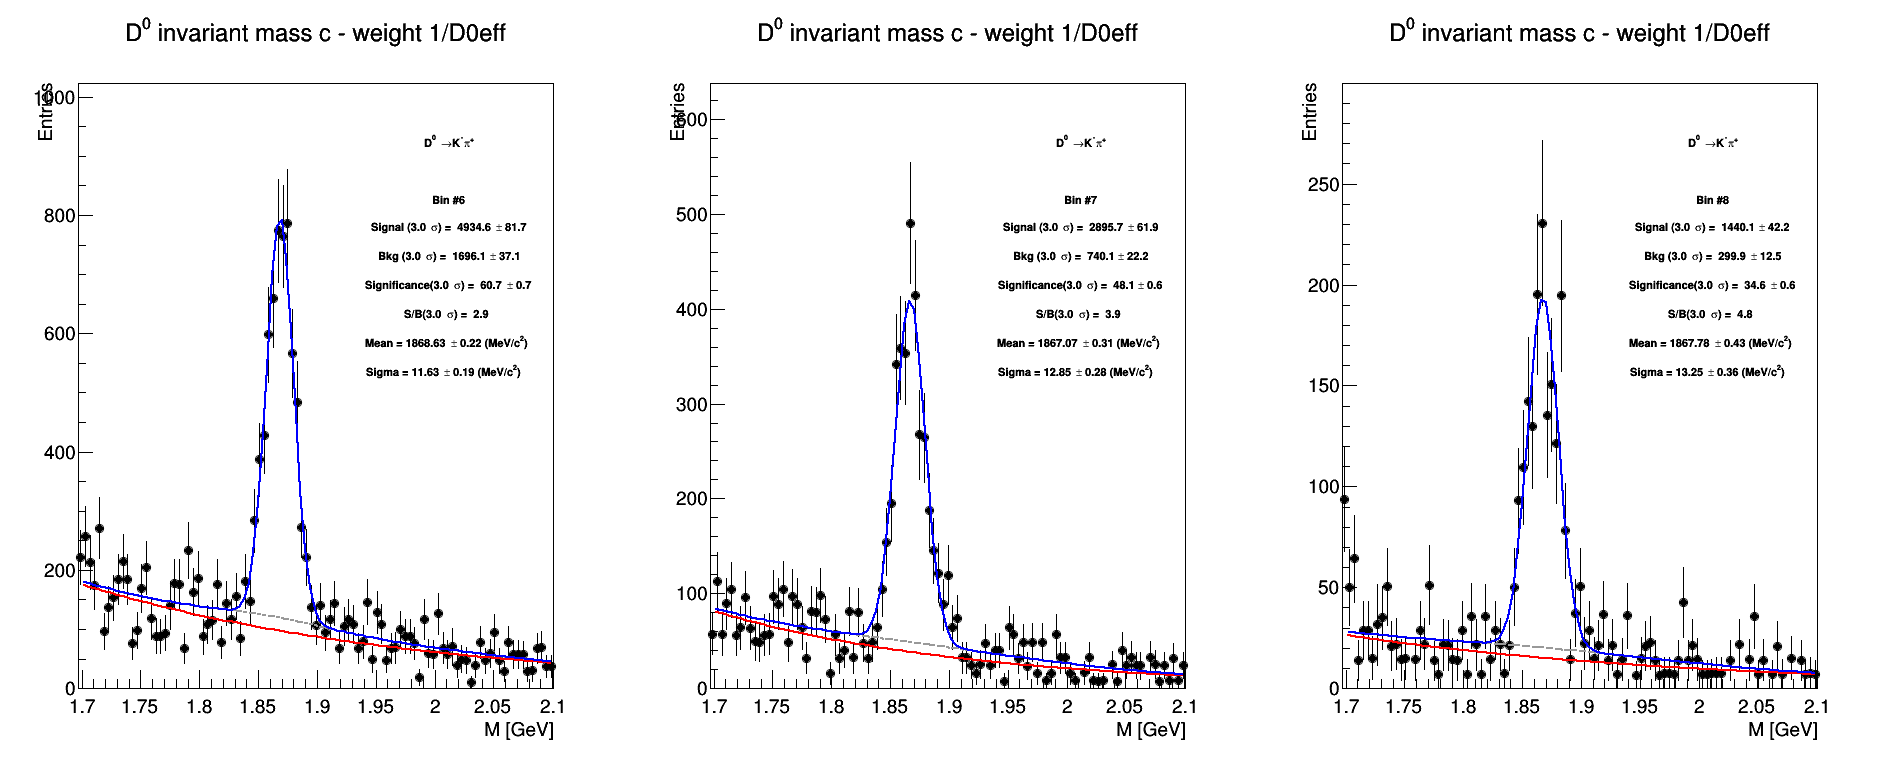
\includegraphics[width=1\linewidth, height=5.6cm]{figuresVsCent/Dzero/MassPlots/60100/InvMassDistributions_Dzero_Bins6to8.png}}
{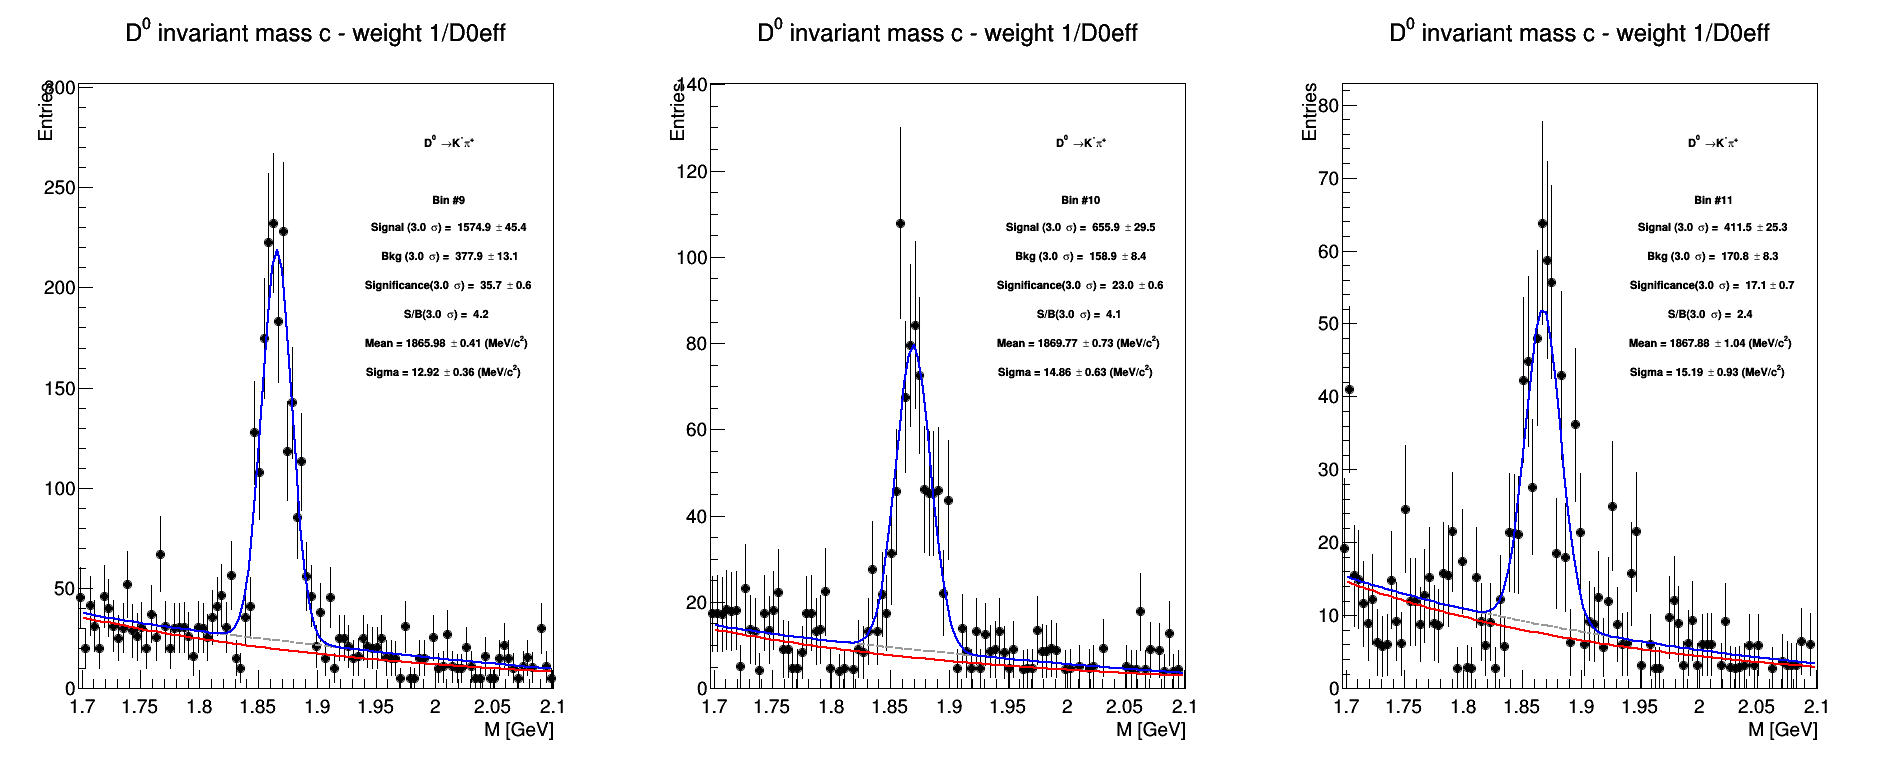
\includegraphics[width=1\linewidth, height=5.6cm]{figuresVsCent/Dzero/MassPlots/60100/InvMassDistributions_Dzero_Bins9to11.png}}
{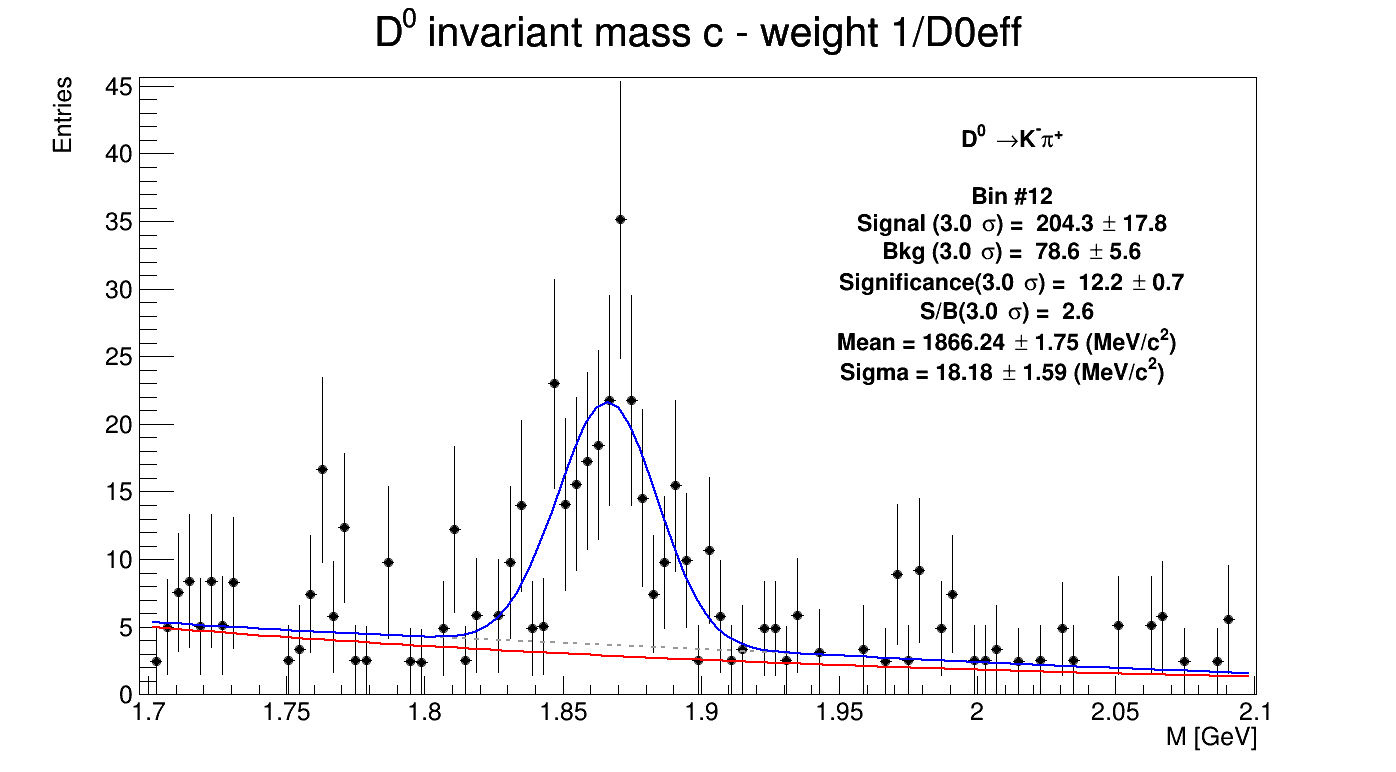
\includegraphics[width=0.6\linewidth, height=5.6cm]{figuresVsCent/Dzero/MassPlots/60100/InvMassDistributions_Dzero_Bins12to12.png}}

%[width=.32\linewidth]
\caption{Invariant mass distributions of $D^0$ corrected with efficiency in different $\text{p}_T$ regions for 60-100$\%$ centrality class. Top: $3< p_{T}^{\text{D}}< 4$ $\gev/c$ (left), $4< p_{T}^{\text{D}}< 5$ $\gev/c$ right), Mid 1: $5< p_{T}^{\text{D}}< 6$ $\gev/c$ (left), $6 < p_{T}^{\text{D}} < 7$ $\gev/c$ (middle), $7< p_{T}^{\text{D}}< 8$ $\gev/c$ (right); Mid2: $8< p_{T}^{\text{D}}< 10$ $\gev/c$, $10< p_{T}^{\text{D}}< 12$ $\gev/c$  (middle), $12 < p_{T}^{\text{D}}< 16$ $\gev/c$  (right) and Bottom: $16<p_{T}^{\text{D}}< 24$ $\gev/c$.}
\label{fig:InvMassD060100}
\end{figure}


\begin{figure}[!htp]
\centering
{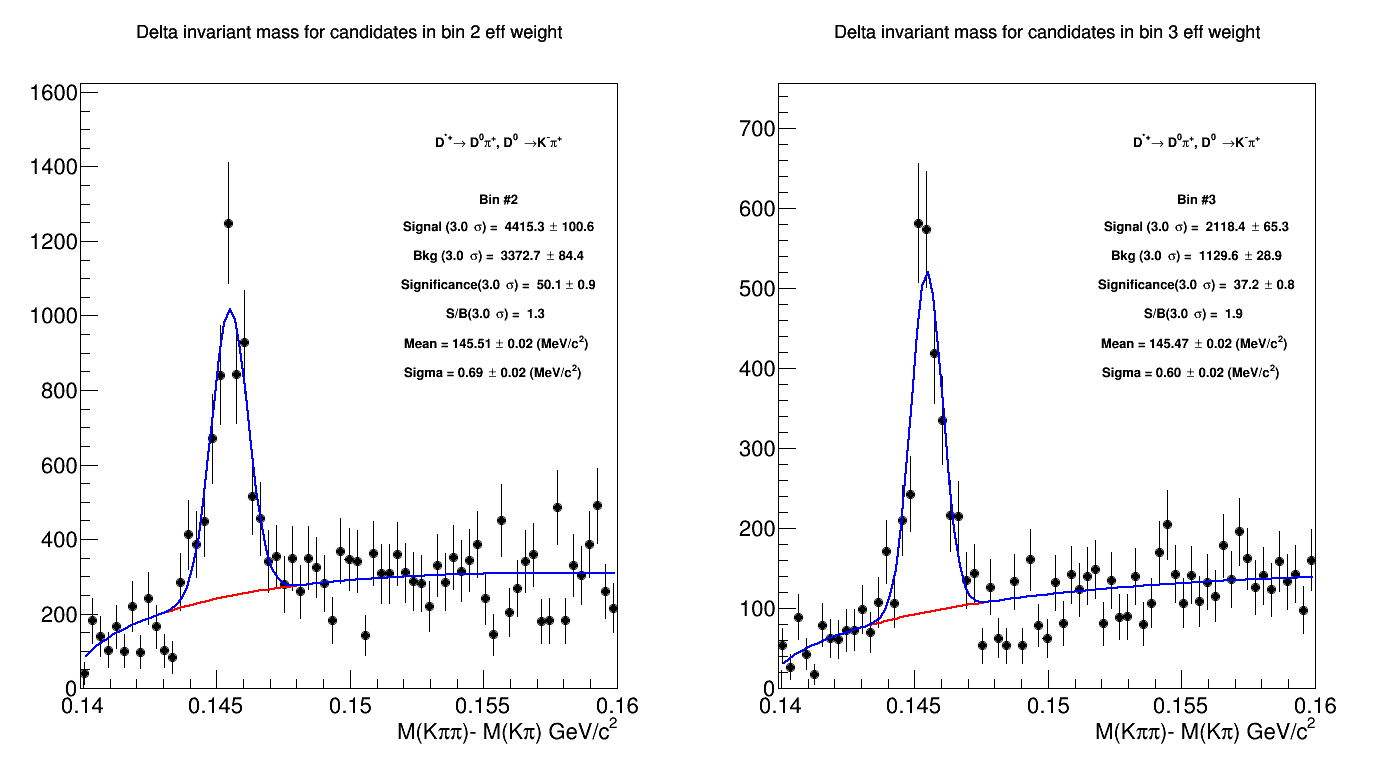
\includegraphics[width=1\linewidth, height=5.6cm]{figuresVsCent/Dstar/MassPlots/60100/InvMassDistributions_Dstar_Bins2to3.png}}
{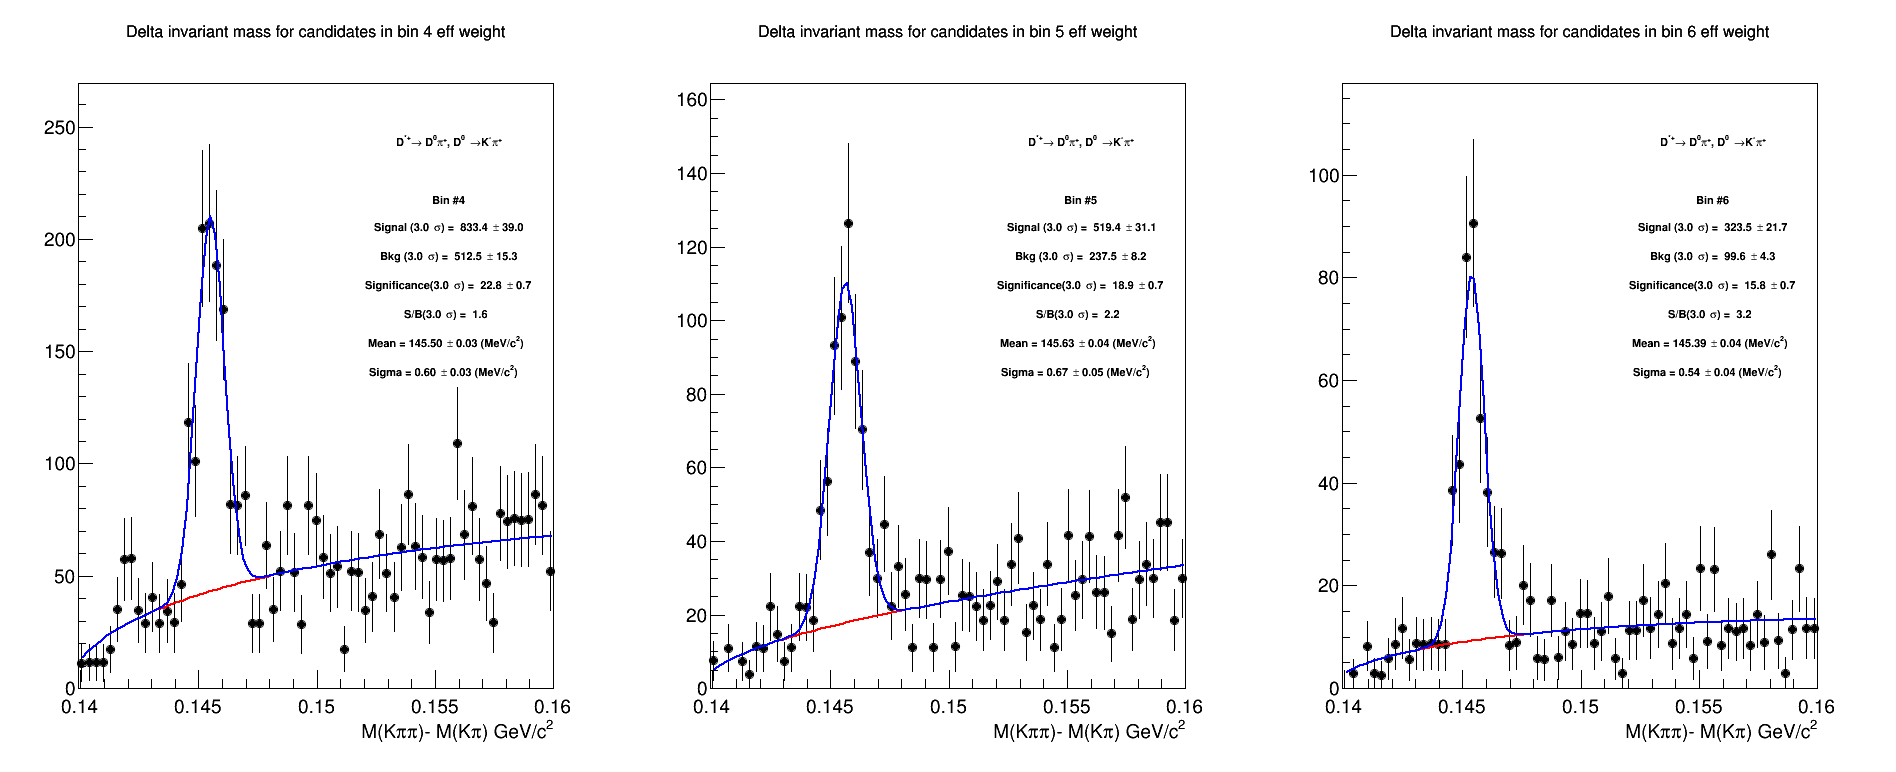
\includegraphics[width=1\linewidth, height=5.6cm]{figuresVsCent/Dstar/MassPlots/60100/InvMassDistributions_Dstar_Bins4to6.png}}
{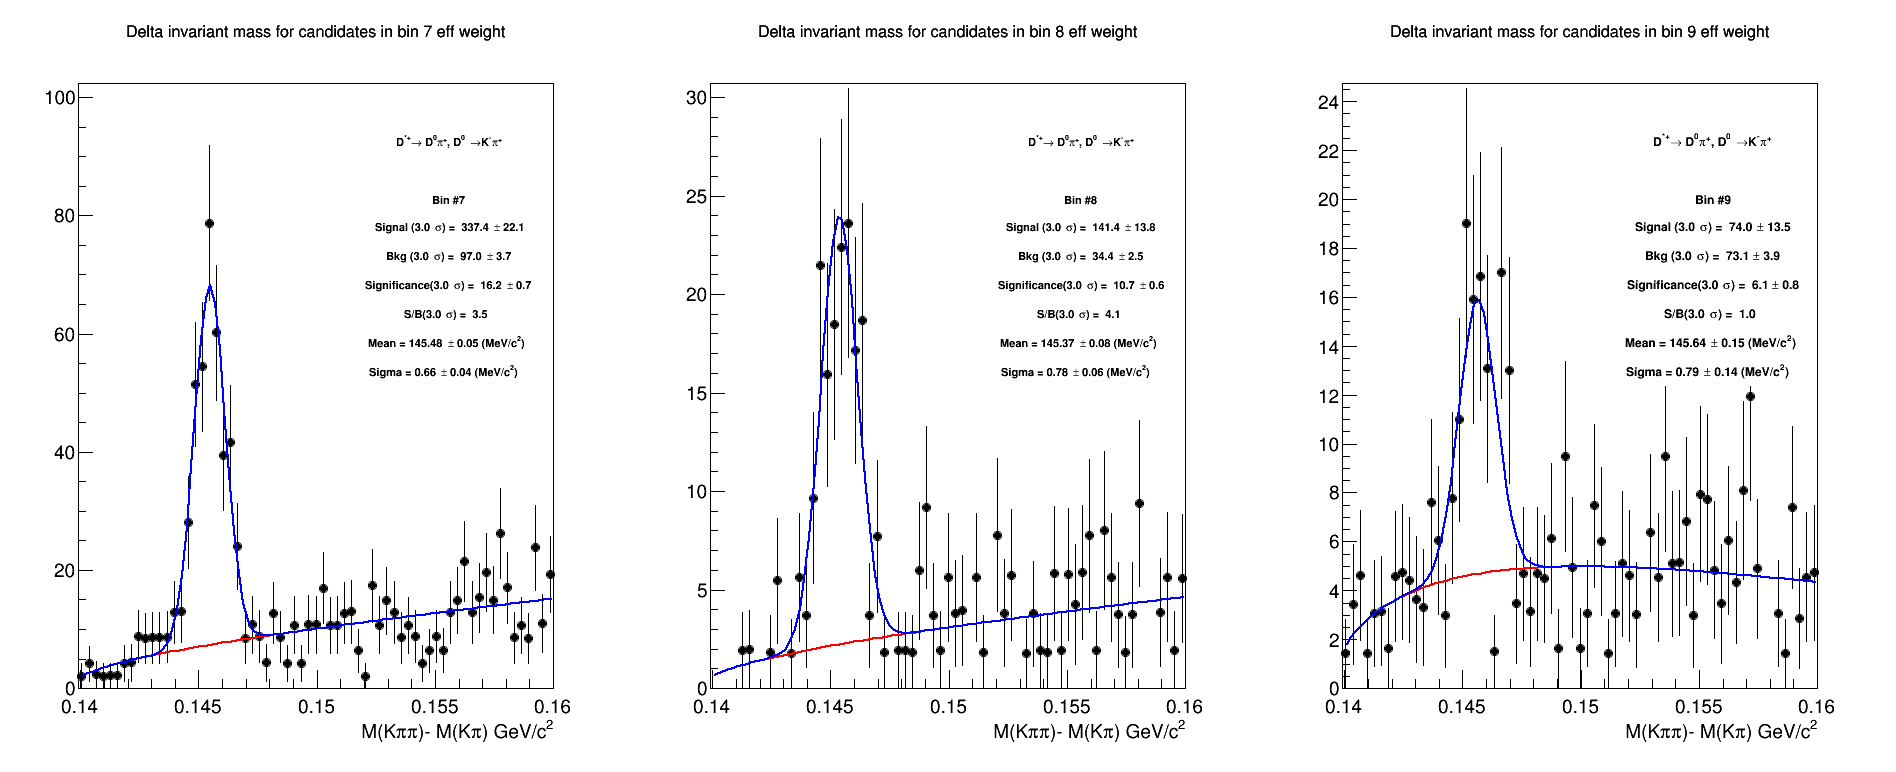
\includegraphics[width=1\linewidth, height=5.6cm]{figuresVsCent/Dstar/MassPlots/60100/InvMassDistributions_Dstar_Bins7to9.png}}
{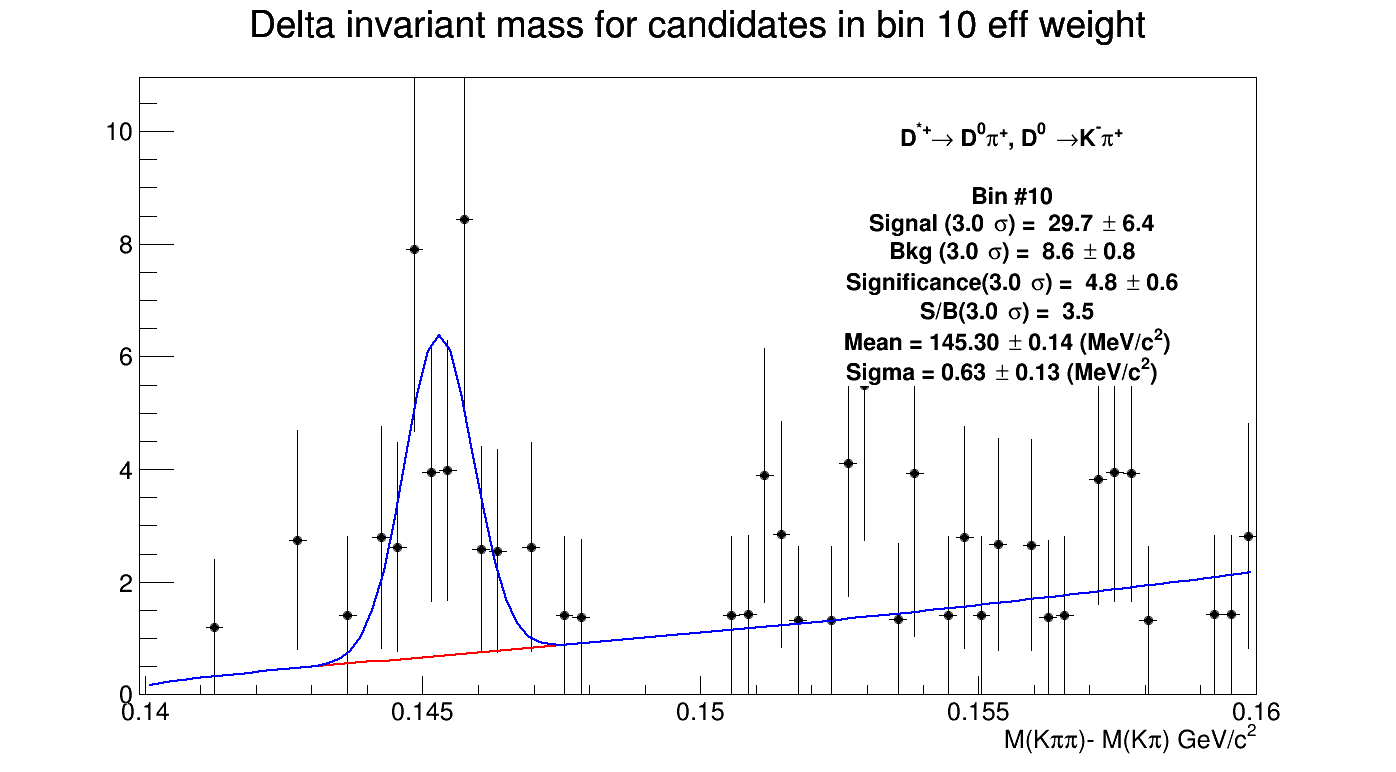
\includegraphics[width=0.6\linewidth, height=5.6cm]{figuresVsCent/Dstar/MassPlots/60100/InvMassDistributions_Dstar_Bins10to10.png}}

\caption{Invariant mass distributions of $\Dstar$ corrected with efficiency in different $\text{p}_T$ regions for 60-100$\%$ centrality class. Top: $3< p_{T}^{\text{D}}< 4$ $\gev/c$ (left), $4< p_{T}^{\text{D}}< 5$ $\gev/c$ right), Mid 1: $5< p_{T}^{\text{D}}< 6$ $\gev/c$ (left), $6 < p_{T}^{\text{D}} < 7$ $\gev/c$ (middle), $7< p_{T}^{\text{D}}< 8$ $\gev/c$ (right); Mid2: $8< p_{T}^{\text{D}}< 10$ $\gev/c$, $10< p_{T}^{\text{D}}< 12$ $\gev/c$  (middle), $12 < p_{T}^{\text{D}}< 16$ $\gev/c$  (right) and Bottom: $16<p_{T}^{\text{D}}< 24$ $\gev/c$ .}
\label{fig:InvMassDs60100}
\end{figure}



\begin{figure}[!htp]
\centering
{\includegraphics[width=1\linewidth, height=5.6cm]{Centrality_DPlus/Dplus/Cmp_Prompt/ZNA/60_100/DplusMassPlots/
/InvMassDistributions_Dstar_Bins3to4.png}}
{\includegraphics[width=1\linewidth, height=5.6cm]{Centrality_DPlus/Dplus/Cmp_Prompt/ZNA/60_100/DplusMassPlots/
/InvMassDistributions_Dstar_Bins5to7.png}}
{\includegraphics[width=1\linewidth, height=5.6cm]{Centrality_DPlus/Dplus/Cmp_Prompt/ZNA/60_100/DplusMassPlots/
/InvMassDistributions_Dstar_Bins8to10.png}}
{\includegraphics[width=0.6\linewidth, height=5.6cm]{Centrality_DPlus/Dplus/Cmp_Prompt/ZNA/60_100/DplusMassPlots/
/InvMassDistributions_Dstar_Bins11to11.png}}

\caption{Invariant mass distributions of $\Dplus$ corrected with efficiency in different $\text{p}_T$ regions for 60-100$\%$ centrality class. Top: $3< p_{T}^{\text{D}}< 4$ $\gev/c$ (left), $4< p_{T}^{\text{D}}< 5$ $\gev/c$ right), Mid 1: $5< p_{T}^{\text{D}}< 6$ $\gev/c$ (left), $6 < p_{T}^{\text{D}} < 7$ $\gev/c$ (middle), $7< p_{T}^{\text{D}}< 8$ $\gev/c$ (right); Mid2: $8< p_{T}^{\text{D}}< 10$ $\gev/c$, $10< p_{T}^{\text{D}}< 12$ $\gev/c$  (middle), $12 < p_{T}^{\text{D}}< 16$ $\gev/c$  (right) and Bottom: $16<p_{T}^{\text{D}}< 24$ $\gev/c$ .}
\label{fig:InvMassDplus60100}
\end{figure}



\subsubsection{Event mixing}
- dire la pool configuration vs cent

\subsubsection{Trigger and tracking efficiency}
- dire strategia di ripesaggio

\subsubsection{Feed-down correction}
- dire le ipotesi sottostanti (mio talk)
- mostrare gli fprompt

\subsubsection{Purity correction}
- dire i valori di purity
- dire vs deltaphi

\subsubsection{Correction for bias on B to D decay topologies}
- dire il MC closure test vs centrality e le features (mio talk)
